%==============================================================================
% ETHASL - Template for student projects at the ASL
% 2013.10: Péter Fankhauser
% This template is based on the IMRT Latex template by Eric A. Mueller.
%==============================================================================

\documentclass[10pt,twoside,a4paper]{report}

% ETHASL package
% TODO Choose options according to your project
% som/bt/st/mt: Studies on Mechatronics, Bachelor Thesis, Semester Thesis, Master Thesis
% fs/hs: Spring term, Autumn term
% german/english: German/English
\usepackage[st,fs,english]{packages/ethasl}

% Activate for german language
%\usepackage{german}
%\usepackage{ae}



%%%%%%%%%%%%%%%%%%%%%%%%%%%%%%%%%%%%%%%%%%%%%%%%%%%%%%%%%%%%%%%%%%%%%%%%%%%%%%%
% LaTeX preamble
%%%%%%%%%%%%%%%%%%%%%%%%%%%%%%%%%%%%%%%%%%%%%%%%%%%%%%%%%%%%%%%%%%%%%%%%%%%%%%%

% URL citing
\usepackage{url}

% SI units
\usepackage{siunitx}

% block diagram with tikz
\usepackage{tikz}
\usepackage{tikzscale}	% includegraphics .tikz
\usetikzlibrary{calc}

% Matrix alligned subfigures
\usepackage[lofdepth,lotdepth]{subfig}

%clock time
\usepackage{datetime}

% matlab2tikz pictures
\usepackage{pgfplots}
% externalize tikz library (faster compilation)
%\usetikzlibrary{external} \tikzexternalize[prefix=tikz/]

% source code
\usepackage{listings}
\lstdefinelanguage{myMatlab}{
	language = Matlab,%    
	basicstyle=\small,%
    breaklines=true,%
    morekeywords={matlab2tikz},
    keywordstyle=\color{blue},%
    morekeywords=[2]{1}, keywordstyle=[2]{\color{black}},
    identifierstyle=\color{black},%
    stringstyle=\color{mylilas},
    commentstyle=\color{mygreen},%
    showstringspaces=false,%without this there will be a symbol in the places where there is a space
    numbers=left,%
    numberstyle={\tiny \color{black}},% size of the numbers
    numbersep=9pt, % this defines how far the numbers are from the text
    emph=[1]{for,end,break},emphstyle=[1]\color{red}, %some words to emphasise
    %emph=[2]{word1,word2}, emphstyle=[2]{style},    
    frame=single,%
}
\lstdefinelanguage{myCVXGEN}{
	language=sh,%
	basicstyle=\small,%
    classoffset=0,%
    morekeywords={dimensions,end,parameters,variables,minimize,subject,to},
    keywordstyle=\color{blue},%
    classoffset=1,%
    morekeywords={diagonal,psd},%
    keywordstyle=\color{darkblue}\it,%
    classoffset=0,%
    moredelim=[s][\color{darkgreen}]{[}{]},%
    moredelim=[s][\color{orange}]{(n}{)},%
    commentstyle=\color{gray},%
    numbers=left,%
    numberstyle={\tiny \color{black}},% size of the numbers
    numbersep=9pt, % this defines how far the numbers are from the text
    frame=single,%
    literate={\ t=0..N}{{\textbf{\textcolor{darkgreen}{\ t=0..N}}}}{7} {\ t=1..N+1}{{\textbf{\textcolor{darkgreen}{\ t=1..N+1}}}}{9} {\ t=0..N-1}{{\textbf{\textcolor{darkgreen}{\ t=0..N-1}}}}{9} {2}{{\textcolor{mypurple}{2}}}{1} {3}{{\textcolor{mypurple}{3}}}{1} {10}{{\textcolor{mypurple}{10}}}{2} {20}{{\textcolor{mypurple}{20}}}{2} {40}{{\textcolor{mypurple}{40}}}{2} {==}{{\textcolor{darkblue}{$==$}}}{2} {<=}{{\textcolor{darkblue}{$<=$}}}{2} {>=}{{\textcolor{darkblue}{$>=$}}}{2} {\ =\ }{{\textcolor{darkgreen}{\ $=$\ }}}{3},%
    moredelim=[s][\color{mypurple}]{\{1,1\ 1,2}{\}},%
    moredelim=[s][\color{mypurple}]{\{5,1}{\}},%
    moredelim=[s][\color{mypurple}]{\{1,1\ 2,1}{\}},%
}

% remarks, theorems etc.
\usepackage{amsthm}
\theoremstyle{remark}
\newtheorem{remark}{Remark}

% larger symbols in math environment for block matrix
\usepackage{relsize}

% algorithms (pseudocode)
\usepackage{algorithm}
\usepackage{algpseudocode}

% cvxcode
\usepackage{upquote}
\definecolor{pdefvalue}{rgb}{0.467,0.000,0.533}
\newcommand{\pdefvalue}[1]{\textcolor{pdefvalue}{#1}}
\definecolor{pdefidentifier}{rgb}{0.000,0.000,0.000}
\newcommand{\pdefidentifier}[1]{\textcolor{pdefidentifier}{#1}}
\definecolor{pdefcomment}{rgb}{0.502,0.502,0.502}
\newcommand{\pdefcomment}[1]{\textcolor{pdefcomment}{#1}}
\definecolor{pdefblock}{rgb}{0.267,0.533,0.867}
\newcommand{\pdefblock}[1]{\textcolor{pdefblock}{#1}}
\definecolor{pdeferror}{rgb}{0.667,0.000,0.000}
\newcommand{\pdeferror}[1]{\textcolor{pdeferror}{#1}}
\definecolor{pdefequals}{rgb}{0.000,0.490,0.000}
\newcommand{\pdefequals}[1]{\textcolor{pdefequals}{#1}}
\definecolor{pdefdim}{rgb}{0.973,0.502,0.090}
\newcommand{\pdefdim}[1]{\textcolor{pdefdim}{#1}}
\definecolor{pdefattr}{rgb}{0.000,0.000,0.467}
\newcommand{\pdefattr}[1]{\textcolor{pdefattr}{#1}}
\definecolor{pdefconstr}{rgb}{0.000,0.000,0.000}
\newcommand{\pdefconstr}[1]{\textcolor{pdefconstr}{#1}}
\definecolor{pdefobjv}{rgb}{0.000,0.000,0.000}
\newcommand{\pdefobjv}[1]{\textcolor{pdefobjv}{#1}}
\definecolor{pdefconstrsign}{rgb}{0.000,0.000,0.800}
\newcommand{\pdefconstrsign}[1]{\textcolor{pdefconstrsign}{#1}}
\definecolor{pdefrange}{rgb}{0.333,0.467,0.200}
\newcommand{\pdefrange}[1]{\textcolor{pdefrange}{#1}}
\definecolor{pdefindex}{rgb}{0.333,0.467,0.200}
\newcommand{\pdefindex}[1]{\textcolor{pdefindex}{#1}}
\definecolor{pdefbrackets}{rgb}{0.333,0.467,0.200}
\newcommand{\pdefbrackets}[1]{\textcolor{pdefbrackets}{#1}}
\definecolor{pdefsemicolon}{rgb}{0.133,0.400,0.800}
\newcommand{\pdefsemicolon}[1]{\textcolor{pdefsemicolon}{#1}}
\definecolor{pdeffunction}{rgb}{0.000,0.333,0.667}
\newcommand{\pdeffunction}[1]{\textcolor{pdeffunction}{#1}}
\definecolor{pdefdenom}{rgb}{0.000,0.333,0.667}
\newcommand{\pdefdenom}[1]{\textcolor{pdefdenom}{#1}}
\definecolor{pdefsparseindices}{rgb}{0.667,0.000,0.533}
\newcommand{\pdefsparseindices}[1]{\textcolor{pdefsparseindices}{#1}}


% colors
\definecolor{mygreen}{RGB}{28,172,0} % color values Red, Green, Blue
\definecolor{mylilas}{RGB}{170,55,241}
\definecolor{mypurple}{RGB}{128,0,128}
\definecolor{myorchid}{RGB}{186,85,211}

% find inkscape pdfs
\graphicspath{{images/}}
% Encoding settings
\usepackage[utf8]{inputenc}
\usepackage[OT1]{fontenc}

% Paper size
\usepackage{a4}

% Headings
\usepackage{fancyhdr}

% More symbols
\usepackage{textcomp}\usepackage{gensymb}

% Math support for Times font
%\usepackage{txfonts}

% ISO date
\usepackage[english]{isodate}

% Multi column
\usepackage{multicol}

% Figures 
\usepackage{graphicx}

% Subfigures (obsolete)
\usepackage{subfig}

% Bibliography
\usepackage[numbers]{natbib}

% Nicer tables
\usepackage{booktabs}
\usepackage{array}
\usepackage{multirow}

% Colors
\usepackage{color}
\usepackage{colortbl}
\definecolor{black}{rgb}{0,0,0}
\definecolor{white}{rgb}{1,1,1}
\definecolor{darkred}{rgb}{0.5,0,0}
\definecolor{darkgreen}{rgb}{0,0.5,0}
\definecolor{darkblue}{rgb}{0,0,0.5}

% Additional math functionality
\usepackage{amsmath}
\usepackage{amssymb}

% Nice fractions
\usepackage{nicefrac}

% Upper case greek letters
\usepackage{upgreek}

% ISO math notation
\usepackage{isomath}
\renewcommand{\vec}{\vectorsym}
\newcommand{\mat}{\matrixsym}

% Units
\usepackage{units}

% Rotated objects
\usepackage{rotating}

% Indent
\setlength{\parindent}{0em}

% Include PDF pages
\usepackage{pdfpages}
\includepdfset{pages={-}, frame=true, pagecommand={\thispagestyle{fancy}}}

% Headings
\rhead[\thepage]{\nouppercase{\rightmark}}
\lhead[\nouppercase{\leftmark}]{\thepage}
\cfoot{}

% Gantt chart
\usepackage{pgfgantt}

% Links (last package)
\usepackage{hyperref}

% Clever references (has to be loaded after hyperref)
\usepackage{cleveref}

%%%%%%%%%%%%%%%%%%%%%%%%%%%%%%%%%%%%%%%%%%%%%%%%%%%%%%%%%%%%%%%%%%%%%%%%%%%%%%%
% Title page
%%%%%%%%%%%%%%%%%%%%%%%%%%%%%%%%%%%%%%%%%%%%%%%%%%%%%%%%%%%%%%%%%%%%%%%%%%%%%%%
\begin{document}

%%%%%%%%%%%%%%%%%%%%%%%%%%%%%%%%%%%%%%%%%%%%%%%%%%%%%%%%%%%%%%%%%%%%%%%%%%%%%%%
% User defined macros
%%%%%%%%%%%%%%%%%%%%%%%%%%%%%%%%%%%%%%%%%%%%%%%%%%%%%%%%%%%%%%%%%%%%%%%%%%%%%%%
\newcommand{\E}{\mathrm{E}}
\newcommand{\Var}{\mathrm{Var}}
\newcommand*\mean[1]{\overline{#1}}
\renewcommand{\d}[1]{\ensuremath{\operatorname{d}\!{#1}}}
\newcommand{\ddt}{\frac{\d{}}{\d{t}}}
\newcommand{\norm}[1]{\left\lVert#1\right\rVert}


\newlength\figureheight 
\newlength\figurewidth
\setlength\figurewidth{0.75\textwidth} 
\setlength\figureheight{0.6\figurewidth} 


% TODO Add your title
\title{Incorporating Aerodynamic Effects into Model Based Control
for Multirotors}
%\subtitle{bla bla bla}

% TODO Add name of the authors
\studentA{Rik M. K. Bähnemann}
%\studentB{Student 2}
% \studentC{Student 3}

% TODO Add name of the supervisors
\supervisionA{Markus Achtelik}
\supervisionB{Michael Burri}
\supervisionC{Mina Kamel}

% TODO Change if necessary
\projectYear{\the\year} % This year
%\projectYear{\advance\year by -1 \the\year\advance\year by 1} % Last year

\maketitle
\pagestyle{plain}
\pagenumbering{roman}

%%%%%%%%%%%%%%%%%%%%%%%%%%%%%%%%%%%%%%%%%%%%%%%%%%%%%%%%%%%%%%%%%%%%%%%%%%%%%%%
% Declaration of originality
%%%%%%%%%%%%%%%%%%%%%%%%%%%%%%%%%%%%%%%%%%%%%%%%%%%%%%%%%%%%%%%%%%%%%%%%%%%%%%%
\pagestyle{empty}

% TODO Modify placeholders in declaration.tex
% TODO Add title, student first/last name, supervisor first/last name.

\section*{Declaration of Originality}

\vspace{1cm}

I hereby declare that the written work I have submitted entitled

\vspace{0.5cm}

% TODO Add title
\textbf{Incorporating Aerodynamic Effects into Model Based Controllers
for Multirotors}

\vspace{0.5cm}

is original work which I alone have authored and which is written in my own words.\footnote{Co-authored work: The signatures of all authors are required. Each signature attests to the originality of the entire piece of written work in its final form.}

\vspace{1cm}

\textbf{Author(s)}

\vspace{0.5cm}

\begin{tabular}{ p{5cm} p{5cm} }
% TODO Add student first/last name
  Rik Marian Kai & Bähnemann \\
\end{tabular}

\supervisionA{Dr. Markus Achtelik}
\supervisionB{Michael Burri}
\supervisionC{Mina Kamel}
\vspace{0.5cm}

\textbf{Student supervisor(s)}

\vspace{0.5cm}

\begin{tabular}{ p{5cm} p{5cm} }
% TODO Add supervisor first/last name
  Markus 		& Achtelik \\
  Michael 		& Burri \\
  Mina		& Kamel \\
\end{tabular}

\vspace{0.5cm}

\textbf{Supervising lecturer}

\vspace{0.5cm}

\begin{tabular}{ p{5cm} p{5cm} }
  Roland & Siegwart \\
\end{tabular}

\vspace{1cm}

With the signature I declare that I have been informed regarding normal academic citation rules and that I have read and understood the information on 'Citation etiquette' (\url{https://www.ethz.ch/content/dam/ethz/associates/students/studium/exams/files-en/plagiarism-citationetiquette.pdf}). The citation conventions usual to the discipline in question here have been respected.

\vspace{0.5cm}

The above written work may be tested electronically for plagiarism.

\vspace{4cm}

\begin{tabular}{ p{5cm} p{1cm} p{5cm} }
  \cline{1-1} \cline{3-3}
  Place and date & & Signature \\
\end{tabular}

%%%%%%%%%%%%%%%%%%%%%%%%%%%%%%%%%%%%%%%%%%%%%%%%%%%%%%%%%%%%%%%%%%%%%%%%%%%%%%%
% Table on contents
%%%%%%%%%%%%%%%%%%%%%%%%%%%%%%%%%%%%%%%%%%%%%%%%%%%%%%%%%%%%%%%%%%%%%%%%%%%%%%%

% Table of Contents depth (TODO change if necessary)
\setcounter{tocdepth}{2}

\tableofcontents
\cleardoublepage

%%%%%%%%%%%%%%%%%%%%%%%%%%%%%%%%%%%%%%%%%%%%%%%%%%%%%%%%%%%%%%%%%%%%%%%%%%%%%%%
% Chapters standard
%%%%%%%%%%%%%%%%%%%%%%%%%%%%%%%%%%%%%%%%%%%%%%%%%%%%%%%%%%%%%%%%%%%%%%%%%%%%%%%
\input{chapters/preface}
\cleardoublepage
\chapter*{Abstract}
\addcontentsline{toc}{chapter}{Abstract}
%\chapter*{Zusammenfassung}
%\addcontentsline{toc}{chapter}{Zusammenfassung}

This semester project addresses the position tracking problem of an unmanned hexacopter under aerodynamic influences. An extended motion model is proposed, which includes drag and wind forces. A cascaded control structure is used to separately control position and attitude. Three controllers for position control are developed: A linear-quadratic regulator, a linear model predictive controller and a nonlinear model predictive controller. Both model predictive controllers are capable of feed-forwarding wind measurements. They also can handle state and actuation constraints and deliver offset-free constant reference tracking. The optimal control problems are solved efficiently using the code generation software CVXGEN and ACADO. The controllers are implemented in MATLAB and tested in various simulated experiments. 
\cleardoublepage
\chapter*{Symbols}
\label{sec:symbols}
\addcontentsline{toc}{chapter}{Symbols}
%\chapter*{Symbolverzeichnis}
%\label{sec:symbole}
%\addcontentsline{toc}{chapter}{Symbolverzeichnis}

\section*{Symbols}
%\section*{Symbole}

\begin{tabbing}
 \hspace*{1.6cm} \= \kill
  $\phi, \theta, \psi$    \> roll, pitch and yaw angle \\[0.5ex] 					
  $b$                     \> gyroscope bias \\[0.5ex]										
  $\Omega_m$              \> 3-axis gyroscope measurement \\[0.5ex]   		
\end{tabbing}

\section*{Indices}
%\section*{Indizes}
\begin{tabbing}
 \hspace*{1.6cm}  \= \kill
 $x$ \> x axis \\[0.5ex]
 $y$ \> y axis \\[0.5ex]
\end{tabbing}

\section*{Acronyms and Abbreviations}
%\section*{Akronyme und Abkürzungen}
\begin{tabbing}
 \hspace*{1.6cm}  \= \kill
 ASL \> Autonomous Systems Lab \\[0.5ex]
 COG \> Center of Gravity \\[0.5ex]
 DoF \> Degrees of Freedom \\[0.5ex]
 ETH \> Eidgenössische Technische Hochschule \\[0.5ex]
 IMU \> Inertial Measurement Unit \\[0.5ex]
 LQR \> Linear-Quadratic Regulator \\[0.5ex]
 MAV \> Micro Aerial Vehicle \\[0.5ex]
 MPC \> Model Predictive Control \\[0.5ex]
 NMPC \> Non-Linear Model Predictive Control \\[0.5ex]
 PEM \> Prediction Error Minimization \\[0.5ex]
 UAV \> Unmanned Aerial Vehicle \\[0.5ex]
 VTOL \> Vertical Take-Off and Landing \\[0.5ex]

\end{tabbing}
\cleardoublepage

%%%%%%%%%%%%%%%%%%%%%%%%%%%%%%%%%%%%%%%%%%%%%%%%%%%%%%%%%%%%%%%%%%%%%%%%%%%%%%%
% Chapters custom
%%%%%%%%%%%%%%%%%%%%%%%%%%%%%%%%%%%%%%%%%%%%%%%%%%%%%%%%%%%%%%%%%%%%%%%%%%%%%%%
\pagestyle{fancy}
\pagenumbering{arabic}

% TODO Add your own chapters here
\chapter{Introduction}
\label{sec:introduction}
%\chapter{Einleitung}
%\label{sec:einleitung}

 Small unmanned aerial vehicles (UAV) have become of major interest both academically and commercially in the last two decades. With the emergence of modern sensor, actuator and computer technology new designs apart from the standard plane and helicopter have been proposed.  Especially multirotor platforms like quad- and hexacopter get a lot of attention these days.

 Multirotors can perform vertical take-off and landing (VTOL) and hovering. With their small size and maneuverability they can be used indoors and outdoors. Unlike helicopters, multirotors can tilt by changing solely the rotor speeds individually. Therefore they do not need mechanical linkages to change the attitude of the rotor blades. This simplifies the design and maintainance and reduces the control problem to calculating appropriate rotor speeds. Paired with sensing, localization and path planning autonomous flight is possible. 

 Not only does this platform motivate research in control theory, computer vision, computer science, and many related fields but it also leads to many commercial applications. 

Amazon Prime Air for example aims at delivering smaller goods with unmanned micro aerial vehicles (MAV) \cite{www:primeair}. Raffaello D'Andrea, professor at ETH Zurich and entrepreneur, predicts that this will be feasible technically as well as economically within the next years \cite{DAndrea2014}. 

Lily is a drone that autonomously films its user, creating unique bird view footage \cite{www:lily}. SenseFly offers drones surveying crops for precision agriculture \cite{www:sensefly}. 3DRobotics sells UAVs for aerial inspection in industry \cite{www:3drobotics}. Other ideas are multi rotors for searching disaster areas, in military, research and, of course, as toys.

Most of these applications require precise position control in order to avoid collisions and meet accuracy requirements. Usually control strategies are based on a simplified mechanical point mass model of the multi rotor. However, these models often neglect aerodynamic influences, like rotor drag, wind or offset of the center of gravity (COG). While this is reasonable at low vehicle speeds, these forces and moments become relevant in more dynamic or outside flights.

The research group around Markus Achtelik at Autonomous Systems Lab (ASL) at ETH Zurich identified dominant dynamics and proposed a extended dynamics model. 

In this student project different model based flight position controllers are proposed that incorporate the effects of rotor drag and wind additionally to the standard model. The controllers are prototyped, simulated and compared in MATLAB. One particular controller is implemented in ROS and simulated in the RotorS simulator. Finally this controller is used on the real MAV in an experiment.

The report will first describe the system dynamics. The equations of motions are derived, the attitude dynamics identified and finally the control system defined. Then the general control scheme is presented and a linear-quadratic regulator (LQR), a linear model predictive controller (MPC) and a non-linear model predictive controller (NMPC) are proposed and simulated in MATLAB. In chapter \ref{sec:rotors} the simulation environment RotorS is described and an implementation of the NMPC is presented. Chapter \ref{sec:experiment} is about a real experiment with the proposed NMPC. Finally conclusions are drawn.
\cleardoublepage
\chapter{Modeling}
\label{sec:modeling}
The position controller proposed in this project will be model based. Therefore we need to define a detailed system which is to be controlled.

In this section the MAV system is stated. It starts by describing the multirotor platform. Then the equations of motion are derived for both translation and rotation. Additionally we include wind into the model. In the fourth part a system identification approach is described to approximate the attitude dynamics. Next the overall dynamics to be controlled are summarized in a system diagram. Finally the system is linearized.

In this project a cascaded control approach is chosen (see figure ). Attitude and motor control run at a high rate ($1000 \si{\hertz}$) in an inner loop, while the high level position controller runs at $100 \si{\hertz}$ in an outer loop. This decoupling is possible because the translational dynamics are much slower than the rotational dynamics. It simplifies the design of the position controller as only translational dynamics have to be considered explicitly and position control reduces to controlling the vehicles desired thrust and direction. 

In order for the vehicle to move to a reference position, the position controller computes the desired thrust force and roll, pitch, yaw angles. The inner loop then takes care of finding the appropriate moment applied to the vehicle body to archive the desired attitude. The attitude controller is given and its dynamics are identified as a linear system.

\begin{figure}
\centering
\includegraphics{images/controller_sketch.tikz}
\caption{Cascaded control sketch}
\label{pics:controller_sketch}
\end{figure}





Also we only consider translational dynamics as they are crucial for position control. The rotational dynamics are handled by the attitude controller. We approximate the closed loop attitude control with a linear system identification.

%%%%%%%%%%%%%%%%%%%%%%%%%%%%%%%%%%%%%%%%%%%%%%%%%%%%%%%%%%%%%%%%%%%%%%%%%%%%%%%
% Platform
%%%%%%%%%%%%%%%%%%%%%%%%%%%%%%%%%%%%%%%%%%%%%%%%%%%%%%%%%%%%%%%%%%%%%%%%%%%%%%%
\section{Platform}
Within this project we use an AscTec Firefly (see figure \ref{pics:firefly}). While this is a hexacopter, the dynamics and controllers are generalized to fit any multirotor configuration. A multirotor is a flying platform consisting of a body and a user specified arrangement of three or more rotors. Only configurations are considered which have all rotors lying fixed in a plane.

In platforms with even-numbered motors, neighboring rotors typically rotate in opposite direction. This compensates yaw moments and gives control over heading. Tilting is accomplished by increasing the thrust on on one side of the vehicle and decreasing it on the opposite side.

The Firefly has six $20 \si{\cm}$ diameter rotors equally aligned around the center. It is $60.5 \times 66.5 \times 16.5 \si{\cm}$ in size and weights $1.6 \si{\kg}$. The maximum thrust is $36 \si{\N}$ and it reaches a maximum airspeed of $15 \si{\metre\per\second}$.

\begin{figure}
   \centering
   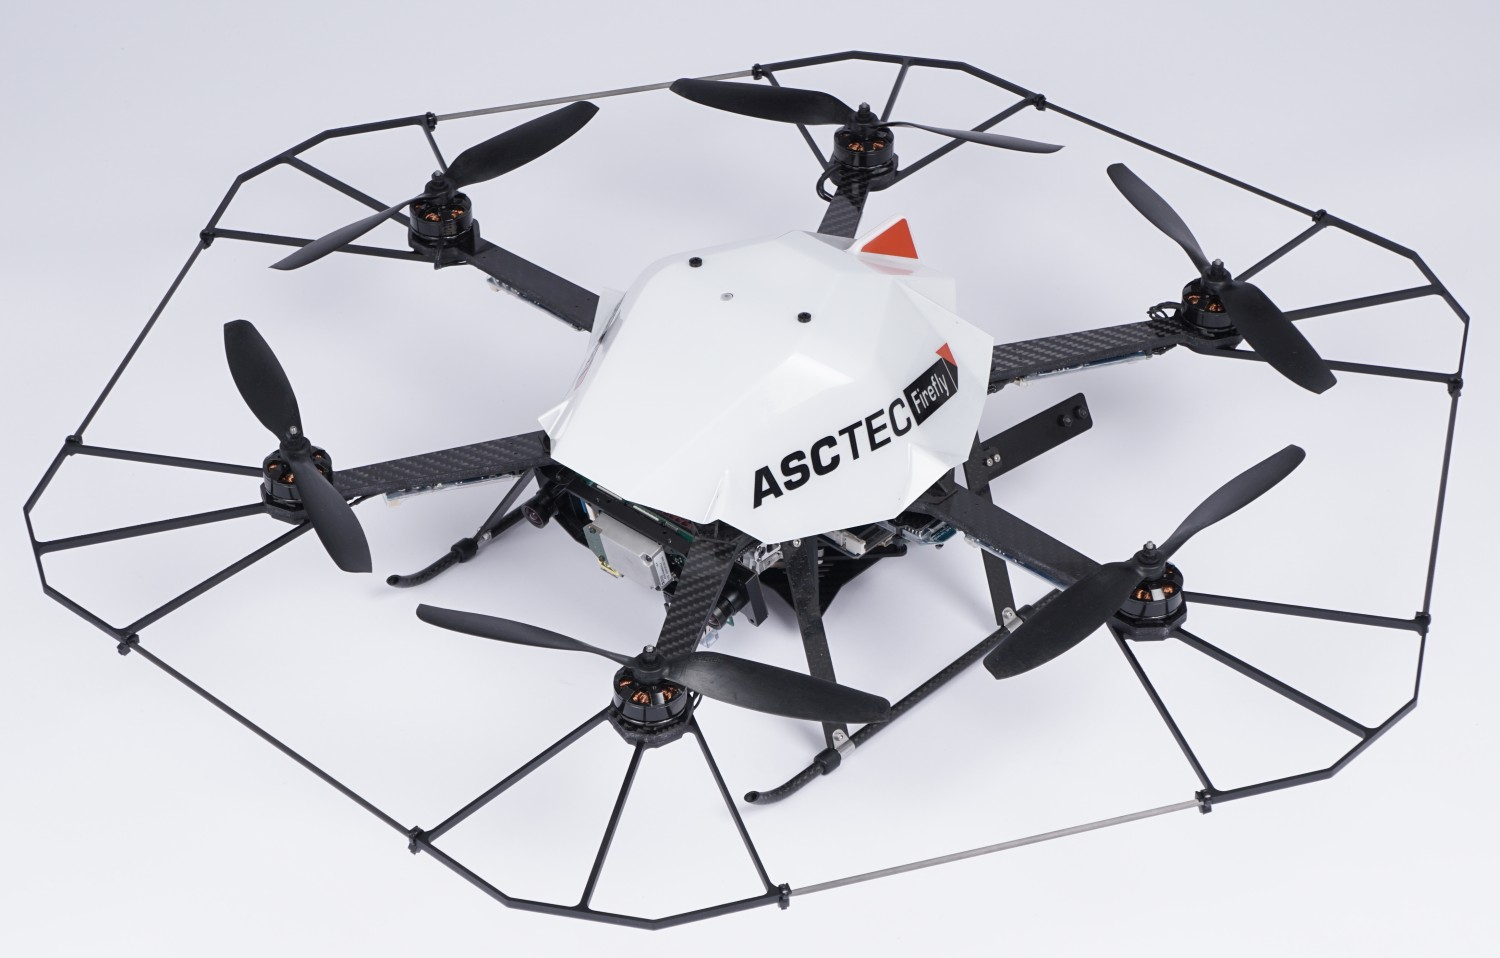
\includegraphics[width=0.75\textwidth]{images/firefly.jpg}
   \caption{AscTec Firefly \cite{www:asctec}}
   \label{pics:firefly}
\end{figure}

It is provided with an inertial measurement unit (IMU) and has a efficient attitude controller onboard. In the experiment an external optical motion capture system by Vicon is used to feedback precise position information. A processor is taking care of online computation.

%%%%%%%%%%%%%%%%%%%%%%%%%%%%%%%%%%%%%%%%%%%%%%%%%%%%%%%%%%%%%%%%%%%%%%%%%%%%%%%
% Equations of Motion
%%%%%%%%%%%%%%%%%%%%%%%%%%%%%%%%%%%%%%%%%%%%%%%%%%%%%%%%%%%%%%%%%%%%%%%%%%%%%%%
\section{Equations of Motion}
The multirotor is modeled as a rigid body with six degrees of freedom (DoF). It has three translational DoF $x$, $y$, $z$ and three rotational DoF roll, pitch and yaw ($\phi$, $\theta$, $\psi$).

 For modeling purposes, we define proper reference frames and notations first. Then the dynamics acting at each rotor are stated. Next the Newton's and Euler's equations for the vehicle are formed giving the complete dynamics of the vehicle.

\subsection{Coordinate Systems and Notations}
In total three main reference frames are defined. The inertial frame $W$, an intermediate heading oriented frame $A$ and a body fixed frame $B$. The inertial frame is world fixed with $z$ pointing upwards collinear to the gravitational force. The heading oriented frame $A$ is produced by rotating the world fixed frame around the $z$-axis through the current heading of the MAV. The body fixed frame is produced by rotating frame $A$ first through the pitch angle about the $y$-axis and then through the roll angle about the $x$-axis. This corresponds to Tait-Bryan angles or $zyx$-sequence. It is located at the body's principal axes of inertia.

We denote vectors and matrices with a bold letter. A leading subscript on a vector denotes the corresponding coordinate frame. A leading double subscript on a matrix denotes the coordinate transformation from the second subscript frame to the first subscript frame. A single trailing subscript serves as additional discriptor. We abbreviate $\sin(\cdot)$ and $\cos(\cdot)$ with $s \cdot$ or $c \cdot$ respectively.

For the rotations we get
\begin{align}
_{BW}\mathbf{R}_x (\phi)&=  \begin{bmatrix}
1 & 0 & 0 \\
0 & c\phi & s\phi \\
0 & -s\phi & c\phi
\end{bmatrix} ,\\
_{BW}\mathbf{R}_y (\theta)&=  \begin{bmatrix}
c\theta & 0 & -s\theta \\
0 & 1 & 0 \\
s\theta & 0 & c\theta
\end{bmatrix} ,\\
_{BW}\mathbf{R}_z (\psi)&=  \begin{bmatrix}
c\psi & s\psi & 0 \\
-s\psi & c\psi & 0 \\
0 & 0 &1
\end{bmatrix}.
\end{align}

Vectors in world frame can then be transformed into body frame and back with
\begin{align}
_{BW}\mathbf{R} (\phi,\theta,\psi) &= {_{BW}\mathbf{R}_x} (\phi) \cdot {_{BW}\mathbf{R}_y} (\theta) \cdot {_{BW}\mathbf{R}_z} (\psi) \\
&=
 \begin{bmatrix}
c\theta c\psi 				&c\theta s\psi 				& -s\theta  \\
s\phi s\theta c\psi - c\phi s\psi  	& s\phi s\theta s\psi + c\phi c\psi 	& s\phi c\theta \\
c\phi s\theta c\psi + s\phi s\psi	& c\phi s\theta s\psi - s\phi c\psi 	& c\phi c\theta
\end{bmatrix} ,\\
_{WB}\mathbf{R} (\phi,\theta,\psi) &= {_{BW}\mathbf{R} (\phi,\theta,\psi)}^{-1} = {_{BW}\mathbf{R} (\phi,\theta,\psi)}^{T} \\
&=
\begin{bmatrix}
c\theta c\psi & s\phi s\theta c\psi - c\phi s\psi & c\phi s\theta c\psi + s\phi s\psi \\
c\theta s\psi & s\phi s\theta s\psi + c\phi c\psi & c\phi s\theta s\psi - s\phi c\psi \\
-s\theta & s\phi c\theta & c\phi c\theta
\end{bmatrix}.
\end{align}

Rotations from the inertial frame to the intermediate heading oriented frame and back are done via
\begin{align}
_{AW}\mathbf{R} (\psi) &= {_{BW}\mathbf{R}_z} (\psi) ,\\
_{WA}\mathbf{R} (\psi) &= {_{AW}\mathbf{R} (\psi)}^{-1} = {_{AW}\mathbf{R} (\psi)}^{T}.
\end{align}

And finally rotations from the intermediate frame to the body frame are
\begin{align}
_{BA}\mathbf{R} (\phi,\theta) &= {_{BW}\mathbf{R}_x} (\phi) \cdot {_{BW}\mathbf{R}_y} (\theta)  ,\\
_{AB}\mathbf{R} (\phi,\theta) &= {_{BA}\mathbf{R} (\phi,\theta)}^{-1} = {_{BA}\mathbf{R} (\phi,\theta)}^{T}.
\end{align}


\subsection{Dynamics}
Martin et al. \cite{Martin2010} propose that the dominant forces and moments acting on a regular multirotor origin from the summation of the aerodynamic effects at each rotor and the gravitational force. We state the rotor dynamics with equations \ref{eq:rotor_begin} to \ref{eq:rotor_begin} which eventually lead to the Newton's equation \ref{eq:newton} and Euler's equation \ref{eq:euler} which completely describe the vehicle equations of motion. We do not model motor dynamics as they are much faster than the translational dynamics.

\subsubsection{Rotor Dynamics}
Blade theory gives the mechanics of each propeller/motor assembly. We neglect 
\begin{itemize} 
\item blade flapping (stiff rotors),
\item high order linear and angular velocity terms (small at hovering compared to blade tip speed),
\item linear and angular acceleration of propellers (low mass),
\item angular acceleration of motors (small at hovering),
\item friction torque due to rotational motion.
\end{itemize}

The remaining major forces are thrust $F_T$ and drag $F_D$. Thrust acts perpendicular to the blade plane and lifts the body. Drag acts opposing to the vehicle's airspeed and slows down the vehicle. The major torques acting on a single blade are roll moments $M_R$ and drag moments $M_D$. The direction of these moments and forces are depicted in figure. 

\begin{align}
\mathbf{F}_T&= \omega^2 \cdot C_T \cdot _B\mathbf{e}_z  &\text{(thrust)} ,\label{eq:rotor_begin} \\
\mathbf{F}_D&= -\omega \cdot  C_D \cdot _B\mathbf{\boldsymbol{\nu}}^\perp  &\text{(drag)} , \label{eq:drag_force}\\
\mathbf{M}_R&= \omega \cdot C_R \cdot _B\mathbf{\boldsymbol{\nu}}^\perp &\text{(roll)} , \\
\mathbf{M}_D&= -\epsilon \cdot C_M \cdot \mathbf{F_T}  &\text{(drag)}, \label{eq:rotor_end}
\end{align}
where
\begin{align*}
\omega &: &\text{angular velocity of rotor blade}, \\
C_T>0 &: &\text{thrust constant}, \\
C_D>0 &: &\text{drag constant}, \\
C_R>0 &: &\text{rolling moment constant}, \\
C_M>0 &: &\text{drag moment constant}, \\
\epsilon\in\{-1,1\} &: &\text{turning direction (clockwise, counter clockwise)}, \\
_B\mathbf{e}_z &: &\text{unit vector in z-direction in base coordinates},\\
_B\mathbf{\boldsymbol{\nu}} &: &\text{airspeed in base coordinates} .
\end{align*}

The $\perp$-symbol denotes the projection of the air speed on the propeller plane (see figure). It can be calculated as:

\begin{align}
_B\mathbf{\boldsymbol{\nu}}^\perp = _B\mathbf{e}_z \times (_B\mathbf{\boldsymbol{\nu}} \times _B\mathbf{e}_z) = _B\mathbf{\boldsymbol{\nu}} - ( _B\mathbf{\boldsymbol{\nu}} \cdot _B\mathbf{e}_z) \cdot _B\mathbf{e}_z .
\end{align}

\subsubsection{Newton's Equations}
The acceleration $\mathbf{a}$ in world frame can be found using Newton's second law. The sum of all forces acting induced by the $n$ rotors and the gravitational force $\mathbf{F}_G$ equals to the body mass $m$ multiplied with the body acceleration.
\begin{align}
\mathbf{F} = m \cdot \mathbf{a} = _{WB}\mathbf{R} \sum_{i=1}^n \underbrace{\left(\mathbf{F}_{T,i} + \mathbf{F}_{D,i} \right)}_{=:\mathbf{F}_i} + \mathbf{F}_G \label{eq:newton}
\end{align}

\subsubsection{Euler's Equations}
The torque $\boldsymbol{\tau}$ acting on vehicle body's base can be found using Euler's equations for rigid body dynamics.
\begin{align}
\boldsymbol{\tau} = \mathbf{J} \cdot  \mathbf{\dot{\boldsymbol{\omega}}} + \boldsymbol{\omega} \times \mathbf{J} \cdot \boldsymbol{\omega} = \sum_{i=1}^n \left( \mathbf{M}_{R,i}+ \mathbf{M}_{D,i} + \mathbf{F}_i \times \mathbf{r}_i \right)  \label{eq:euler}
\end{align}
$\mathbf{J}$  is the inertia matrix referenced to the center of mass along the base frame. $\mathbf{r}_i$ denotes the vector from the CoG of the MAV to the $i$-th rotor. $\boldsymbol{\omega}$ is the angular velocity about the same frame. For small tilt angles the angular velocity is approximately equal to the change in Euler angles in which the system is described.
\begin{align}
\boldsymbol{\omega} \approx \begin{bmatrix}
\dot\phi \\ \dot\theta \\ \dot\psi
\end{bmatrix}
\end{align}


The moment equations are dispensible, because attitude control is taken care of by an implemented controller already and its closed loop dynamics will be identified below. We still write them down for completeness.

%%%%%%%%%%%%%%%%%%%%%%%%%%%%%%%%%%%%%%%%%%%%%%%%%%%%%%%%%%%%%%%%%%%%%%%%%%%%%%%
% Wind effects
%%%%%%%%%%%%%%%%%%%%%%%%%%%%%%%%%%%%%%%%%%%%%%%%%%%%%%%%%%%%%%%%%%%%%%%%%%%%%%%
\section{Wind Model}
In general wind is neither steady nor constant. Both azimuth and speed tend to jump instantanously. Especially these wind gusts can deflect the MAV dangerously.

Having stated the equations of motion, it is possible to incorporate the effects of wind into the dynamics. This can help improve the controller performance in the case of a wind gust. If the wind is measured or known, the controller can feedforward the effects.

\subsection{Wind Dynamics}
Gust is usually defined as a increase of wind velocity $\mathbf{w}$ by $5\si{\metre\per\second}$ over the $10$-minute average wind velocity and has to have a duration of $3 \si{\second}$ to $20 \si{\second}$.

Figure \ref{fig:wind_observations} shows a typical wind observation. The wind speed is showing random deviation around some time-varying average. From top to bottom the time intervals marked by the vertical grey boxes are magnified to identify short time behaviour.


\begin{figure}
\centering
\subfloat[][{$24\si{\hour}$ wind speed $[ \si{\metre\per\second} ]$ observation }]{
% GNUPLOT: LaTeX picture with Postscript
\begingroup
  \makeatletter
  \providecommand\color[2][]{%
    \GenericError{(gnuplot) \space\space\space\@spaces}{%
      Package color not loaded in conjunction with
      terminal option `colourtext'%
    }{See the gnuplot documentation for explanation.%
    }{Either use 'blacktext' in gnuplot or load the package
      color.sty in LaTeX.}%
    \renewcommand\color[2][]{}%
  }%
  \providecommand\includegraphics[2][]{%
    \GenericError{(gnuplot) \space\space\space\@spaces}{%
      Package graphicx or graphics not loaded%
    }{See the gnuplot documentation for explanation.%
    }{The gnuplot epslatex terminal needs graphicx.sty or graphics.sty.}%
    \renewcommand\includegraphics[2][]{}%
  }%
  \providecommand\rotatebox[2]{#2}%
  \@ifundefined{ifGPcolor}{%
    \newif\ifGPcolor
    \GPcolortrue
  }{}%
  \@ifundefined{ifGPblacktext}{%
    \newif\ifGPblacktext
    \GPblacktextfalse
  }{}%
  % define a \g@addto@macro without @ in the name:
  \let\gplgaddtomacro\g@addto@macro
  % define empty templates for all commands taking text:
  \gdef\gplbacktext{}%
  \gdef\gplfronttext{}%
  \makeatother
  \ifGPblacktext
    % no textcolor at all
    \def\colorrgb#1{}%
    \def\colorgray#1{}%
  \else
    % gray or color?
    \ifGPcolor
      \def\colorrgb#1{\color[rgb]{#1}}%
      \def\colorgray#1{\color[gray]{#1}}%
      \expandafter\def\csname LTw\endcsname{\color{white}}%
      \expandafter\def\csname LTb\endcsname{\color{black}}%
      \expandafter\def\csname LTa\endcsname{\color{black}}%
      \expandafter\def\csname LT0\endcsname{\color[rgb]{1,0,0}}%
      \expandafter\def\csname LT1\endcsname{\color[rgb]{0,1,0}}%
      \expandafter\def\csname LT2\endcsname{\color[rgb]{0,0,1}}%
      \expandafter\def\csname LT3\endcsname{\color[rgb]{1,0,1}}%
      \expandafter\def\csname LT4\endcsname{\color[rgb]{0,1,1}}%
      \expandafter\def\csname LT5\endcsname{\color[rgb]{1,1,0}}%
      \expandafter\def\csname LT6\endcsname{\color[rgb]{0,0,0}}%
      \expandafter\def\csname LT7\endcsname{\color[rgb]{1,0.3,0}}%
      \expandafter\def\csname LT8\endcsname{\color[rgb]{0.5,0.5,0.5}}%
    \else
      % gray
      \def\colorrgb#1{\color{black}}%
      \def\colorgray#1{\color[gray]{#1}}%
      \expandafter\def\csname LTw\endcsname{\color{white}}%
      \expandafter\def\csname LTb\endcsname{\color{black}}%
      \expandafter\def\csname LTa\endcsname{\color{black}}%
      \expandafter\def\csname LT0\endcsname{\color{black}}%
      \expandafter\def\csname LT1\endcsname{\color{black}}%
      \expandafter\def\csname LT2\endcsname{\color{black}}%
      \expandafter\def\csname LT3\endcsname{\color{black}}%
      \expandafter\def\csname LT4\endcsname{\color{black}}%
      \expandafter\def\csname LT5\endcsname{\color{black}}%
      \expandafter\def\csname LT6\endcsname{\color{black}}%
      \expandafter\def\csname LT7\endcsname{\color{black}}%
      \expandafter\def\csname LT8\endcsname{\color{black}}%
    \fi
  \fi
  \setlength{\unitlength}{0.0500bp}%
  \begin{picture}(3454.00,1700.00)%
    \gplgaddtomacro\gplbacktext{%
      \csname LTb\endcsname%
      \put(594,484){\makebox(0,0)[r]{\strut{} 0}}%
      \put(594,722){\makebox(0,0)[r]{\strut{} 4}}%
      \put(594,960){\makebox(0,0)[r]{\strut{} 8}}%
      \put(594,1197){\makebox(0,0)[r]{\strut{} 12}}%
      \put(594,1435){\makebox(0,0)[r]{\strut{} 16}}%
      \put(726,264){\makebox(0,0){\strut{}00}}%
      \put(1309,264){\makebox(0,0){\strut{}06}}%
      \put(1892,264){\makebox(0,0){\strut{}12}}%
      \put(2474,264){\makebox(0,0){\strut{}18}}%
      \put(3057,264){\makebox(0,0){\strut{}00}}%
      \put(1891,154){\makebox(0,0){\strut{}time $[\si{\hour}]$}}%
    }%
    \gplgaddtomacro\gplfronttext{%
    }%
    \gplbacktext
    \put(0,0){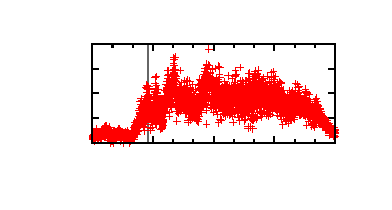
\includegraphics{/home/rik/workspace/ASL_student_project/Repositories/report-fork/Presentation/LaTeX_Template/images/windday}}%
    \gplfronttext
  \end{picture}%
\endgroup

\label{fig:wind_speed_day}}
\subfloat[][{$24\si{\hour}$ wind azimuth $[ \si{\degree} ]$ observation}]{
% GNUPLOT: LaTeX picture with Postscript
\begingroup
  \makeatletter
  \providecommand\color[2][]{%
    \GenericError{(gnuplot) \space\space\space\@spaces}{%
      Package color not loaded in conjunction with
      terminal option `colourtext'%
    }{See the gnuplot documentation for explanation.%
    }{Either use 'blacktext' in gnuplot or load the package
      color.sty in LaTeX.}%
    \renewcommand\color[2][]{}%
  }%
  \providecommand\includegraphics[2][]{%
    \GenericError{(gnuplot) \space\space\space\@spaces}{%
      Package graphicx or graphics not loaded%
    }{See the gnuplot documentation for explanation.%
    }{The gnuplot epslatex terminal needs graphicx.sty or graphics.sty.}%
    \renewcommand\includegraphics[2][]{}%
  }%
  \providecommand\rotatebox[2]{#2}%
  \@ifundefined{ifGPcolor}{%
    \newif\ifGPcolor
    \GPcolortrue
  }{}%
  \@ifundefined{ifGPblacktext}{%
    \newif\ifGPblacktext
    \GPblacktextfalse
  }{}%
  % define a \g@addto@macro without @ in the name:
  \let\gplgaddtomacro\g@addto@macro
  % define empty templates for all commands taking text:
  \gdef\gplbacktext{}%
  \gdef\gplfronttext{}%
  \makeatother
  \ifGPblacktext
    % no textcolor at all
    \def\colorrgb#1{}%
    \def\colorgray#1{}%
  \else
    % gray or color?
    \ifGPcolor
      \def\colorrgb#1{\color[rgb]{#1}}%
      \def\colorgray#1{\color[gray]{#1}}%
      \expandafter\def\csname LTw\endcsname{\color{white}}%
      \expandafter\def\csname LTb\endcsname{\color{black}}%
      \expandafter\def\csname LTa\endcsname{\color{black}}%
      \expandafter\def\csname LT0\endcsname{\color[rgb]{1,0,0}}%
      \expandafter\def\csname LT1\endcsname{\color[rgb]{0,1,0}}%
      \expandafter\def\csname LT2\endcsname{\color[rgb]{0,0,1}}%
      \expandafter\def\csname LT3\endcsname{\color[rgb]{1,0,1}}%
      \expandafter\def\csname LT4\endcsname{\color[rgb]{0,1,1}}%
      \expandafter\def\csname LT5\endcsname{\color[rgb]{1,1,0}}%
      \expandafter\def\csname LT6\endcsname{\color[rgb]{0,0,0}}%
      \expandafter\def\csname LT7\endcsname{\color[rgb]{1,0.3,0}}%
      \expandafter\def\csname LT8\endcsname{\color[rgb]{0.5,0.5,0.5}}%
    \else
      % gray
      \def\colorrgb#1{\color{black}}%
      \def\colorgray#1{\color[gray]{#1}}%
      \expandafter\def\csname LTw\endcsname{\color{white}}%
      \expandafter\def\csname LTb\endcsname{\color{black}}%
      \expandafter\def\csname LTa\endcsname{\color{black}}%
      \expandafter\def\csname LT0\endcsname{\color{black}}%
      \expandafter\def\csname LT1\endcsname{\color{black}}%
      \expandafter\def\csname LT2\endcsname{\color{black}}%
      \expandafter\def\csname LT3\endcsname{\color{black}}%
      \expandafter\def\csname LT4\endcsname{\color{black}}%
      \expandafter\def\csname LT5\endcsname{\color{black}}%
      \expandafter\def\csname LT6\endcsname{\color{black}}%
      \expandafter\def\csname LT7\endcsname{\color{black}}%
      \expandafter\def\csname LT8\endcsname{\color{black}}%
    \fi
  \fi
  \setlength{\unitlength}{0.0500bp}%
  \begin{picture}(3454.00,2266.00)%
    \gplgaddtomacro\gplbacktext{%
      \csname LTb\endcsname%
      \put(726,704){\makebox(0,0)[r]{\strut{} 0}}%
      \put(726,1028){\makebox(0,0)[r]{\strut{} 90}}%
      \put(726,1353){\makebox(0,0)[r]{\strut{} 180}}%
      \put(726,1677){\makebox(0,0)[r]{\strut{} 270}}%
      \put(726,2001){\makebox(0,0)[r]{\strut{} 360}}%
      \put(858,484){\makebox(0,0){\strut{}00}}%
      \put(1408,484){\makebox(0,0){\strut{}06}}%
      \put(1958,484){\makebox(0,0){\strut{}12}}%
      \put(2507,484){\makebox(0,0){\strut{}18}}%
      \put(3057,484){\makebox(0,0){\strut{}00}}%
      \put(1957,154){\makebox(0,0){\strut{}time $[\si{\hour}]$}}%
    }%
    \gplgaddtomacro\gplfronttext{%
    }%
    \gplbacktext
    \put(0,0){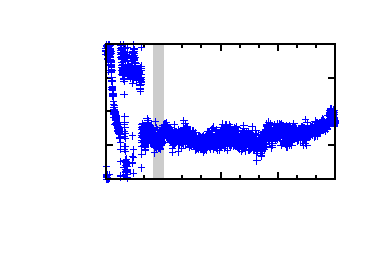
\includegraphics{/home/rik/workspace/ASL_student_project/Repositories/report-fork/Report/images/windaziday}}%
    \gplfronttext
  \end{picture}%
\endgroup

\label{fig:wind_azi_day}}
\qquad
\subfloat[][{Wind speeds $[ \si{\metre\per\second} ]$ from \formattime{5}{0}{0} to \formattime{6}{0}{0} }]{
% GNUPLOT: LaTeX picture with Postscript
\begingroup
  \makeatletter
  \providecommand\color[2][]{%
    \GenericError{(gnuplot) \space\space\space\@spaces}{%
      Package color not loaded in conjunction with
      terminal option `colourtext'%
    }{See the gnuplot documentation for explanation.%
    }{Either use 'blacktext' in gnuplot or load the package
      color.sty in LaTeX.}%
    \renewcommand\color[2][]{}%
  }%
  \providecommand\includegraphics[2][]{%
    \GenericError{(gnuplot) \space\space\space\@spaces}{%
      Package graphicx or graphics not loaded%
    }{See the gnuplot documentation for explanation.%
    }{The gnuplot epslatex terminal needs graphicx.sty or graphics.sty.}%
    \renewcommand\includegraphics[2][]{}%
  }%
  \providecommand\rotatebox[2]{#2}%
  \@ifundefined{ifGPcolor}{%
    \newif\ifGPcolor
    \GPcolortrue
  }{}%
  \@ifundefined{ifGPblacktext}{%
    \newif\ifGPblacktext
    \GPblacktextfalse
  }{}%
  % define a \g@addto@macro without @ in the name:
  \let\gplgaddtomacro\g@addto@macro
  % define empty templates for all commands taking text:
  \gdef\gplbacktext{}%
  \gdef\gplfronttext{}%
  \makeatother
  \ifGPblacktext
    % no textcolor at all
    \def\colorrgb#1{}%
    \def\colorgray#1{}%
  \else
    % gray or color?
    \ifGPcolor
      \def\colorrgb#1{\color[rgb]{#1}}%
      \def\colorgray#1{\color[gray]{#1}}%
      \expandafter\def\csname LTw\endcsname{\color{white}}%
      \expandafter\def\csname LTb\endcsname{\color{black}}%
      \expandafter\def\csname LTa\endcsname{\color{black}}%
      \expandafter\def\csname LT0\endcsname{\color[rgb]{1,0,0}}%
      \expandafter\def\csname LT1\endcsname{\color[rgb]{0,1,0}}%
      \expandafter\def\csname LT2\endcsname{\color[rgb]{0,0,1}}%
      \expandafter\def\csname LT3\endcsname{\color[rgb]{1,0,1}}%
      \expandafter\def\csname LT4\endcsname{\color[rgb]{0,1,1}}%
      \expandafter\def\csname LT5\endcsname{\color[rgb]{1,1,0}}%
      \expandafter\def\csname LT6\endcsname{\color[rgb]{0,0,0}}%
      \expandafter\def\csname LT7\endcsname{\color[rgb]{1,0.3,0}}%
      \expandafter\def\csname LT8\endcsname{\color[rgb]{0.5,0.5,0.5}}%
    \else
      % gray
      \def\colorrgb#1{\color{black}}%
      \def\colorgray#1{\color[gray]{#1}}%
      \expandafter\def\csname LTw\endcsname{\color{white}}%
      \expandafter\def\csname LTb\endcsname{\color{black}}%
      \expandafter\def\csname LTa\endcsname{\color{black}}%
      \expandafter\def\csname LT0\endcsname{\color{black}}%
      \expandafter\def\csname LT1\endcsname{\color{black}}%
      \expandafter\def\csname LT2\endcsname{\color{black}}%
      \expandafter\def\csname LT3\endcsname{\color{black}}%
      \expandafter\def\csname LT4\endcsname{\color{black}}%
      \expandafter\def\csname LT5\endcsname{\color{black}}%
      \expandafter\def\csname LT6\endcsname{\color{black}}%
      \expandafter\def\csname LT7\endcsname{\color{black}}%
      \expandafter\def\csname LT8\endcsname{\color{black}}%
    \fi
  \fi
  \setlength{\unitlength}{0.0500bp}%
  \begin{picture}(3454.00,2266.00)%
    \gplgaddtomacro\gplbacktext{%
      \csname LTb\endcsname%
      \put(594,704){\makebox(0,0)[r]{\strut{} 0}}%
      \put(594,1028){\makebox(0,0)[r]{\strut{} 4}}%
      \put(594,1353){\makebox(0,0)[r]{\strut{} 8}}%
      \put(594,1677){\makebox(0,0)[r]{\strut{} 12}}%
      \put(594,2001){\makebox(0,0)[r]{\strut{} 16}}%
      \put(726,484){\makebox(0,0){\strut{}00}}%
      \put(1309,484){\makebox(0,0){\strut{}15}}%
      \put(1892,484){\makebox(0,0){\strut{}30}}%
      \put(2474,484){\makebox(0,0){\strut{}45}}%
      \put(3057,484){\makebox(0,0){\strut{}00}}%
      \put(1891,154){\makebox(0,0){\strut{}time $[\si{\minute}]$}}%
    }%
    \gplgaddtomacro\gplfronttext{%
    }%
    \gplbacktext
    \put(0,0){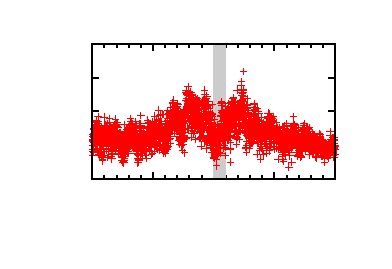
\includegraphics{/home/rik/workspace/ASL_student_project/Repositories/report-fork/Report/images/windhour}}%
    \gplfronttext
  \end{picture}%
\endgroup

\label{fig:wind_speed_hour}}
\subfloat[][{Wind azimuth $[ \si{\degree} ]$ from \formattime{5}{0}{0} to \formattime{6}{0}{0} }]{
% GNUPLOT: LaTeX picture with Postscript
\begingroup
  \makeatletter
  \providecommand\color[2][]{%
    \GenericError{(gnuplot) \space\space\space\@spaces}{%
      Package color not loaded in conjunction with
      terminal option `colourtext'%
    }{See the gnuplot documentation for explanation.%
    }{Either use 'blacktext' in gnuplot or load the package
      color.sty in LaTeX.}%
    \renewcommand\color[2][]{}%
  }%
  \providecommand\includegraphics[2][]{%
    \GenericError{(gnuplot) \space\space\space\@spaces}{%
      Package graphicx or graphics not loaded%
    }{See the gnuplot documentation for explanation.%
    }{The gnuplot epslatex terminal needs graphicx.sty or graphics.sty.}%
    \renewcommand\includegraphics[2][]{}%
  }%
  \providecommand\rotatebox[2]{#2}%
  \@ifundefined{ifGPcolor}{%
    \newif\ifGPcolor
    \GPcolortrue
  }{}%
  \@ifundefined{ifGPblacktext}{%
    \newif\ifGPblacktext
    \GPblacktextfalse
  }{}%
  % define a \g@addto@macro without @ in the name:
  \let\gplgaddtomacro\g@addto@macro
  % define empty templates for all commands taking text:
  \gdef\gplbacktext{}%
  \gdef\gplfronttext{}%
  \makeatother
  \ifGPblacktext
    % no textcolor at all
    \def\colorrgb#1{}%
    \def\colorgray#1{}%
  \else
    % gray or color?
    \ifGPcolor
      \def\colorrgb#1{\color[rgb]{#1}}%
      \def\colorgray#1{\color[gray]{#1}}%
      \expandafter\def\csname LTw\endcsname{\color{white}}%
      \expandafter\def\csname LTb\endcsname{\color{black}}%
      \expandafter\def\csname LTa\endcsname{\color{black}}%
      \expandafter\def\csname LT0\endcsname{\color[rgb]{1,0,0}}%
      \expandafter\def\csname LT1\endcsname{\color[rgb]{0,1,0}}%
      \expandafter\def\csname LT2\endcsname{\color[rgb]{0,0,1}}%
      \expandafter\def\csname LT3\endcsname{\color[rgb]{1,0,1}}%
      \expandafter\def\csname LT4\endcsname{\color[rgb]{0,1,1}}%
      \expandafter\def\csname LT5\endcsname{\color[rgb]{1,1,0}}%
      \expandafter\def\csname LT6\endcsname{\color[rgb]{0,0,0}}%
      \expandafter\def\csname LT7\endcsname{\color[rgb]{1,0.3,0}}%
      \expandafter\def\csname LT8\endcsname{\color[rgb]{0.5,0.5,0.5}}%
    \else
      % gray
      \def\colorrgb#1{\color{black}}%
      \def\colorgray#1{\color[gray]{#1}}%
      \expandafter\def\csname LTw\endcsname{\color{white}}%
      \expandafter\def\csname LTb\endcsname{\color{black}}%
      \expandafter\def\csname LTa\endcsname{\color{black}}%
      \expandafter\def\csname LT0\endcsname{\color{black}}%
      \expandafter\def\csname LT1\endcsname{\color{black}}%
      \expandafter\def\csname LT2\endcsname{\color{black}}%
      \expandafter\def\csname LT3\endcsname{\color{black}}%
      \expandafter\def\csname LT4\endcsname{\color{black}}%
      \expandafter\def\csname LT5\endcsname{\color{black}}%
      \expandafter\def\csname LT6\endcsname{\color{black}}%
      \expandafter\def\csname LT7\endcsname{\color{black}}%
      \expandafter\def\csname LT8\endcsname{\color{black}}%
    \fi
  \fi
  \setlength{\unitlength}{0.0500bp}%
  \begin{picture}(3454.00,2266.00)%
    \gplgaddtomacro\gplbacktext{%
      \csname LTb\endcsname%
      \put(726,704){\makebox(0,0)[r]{\strut{} 0}}%
      \put(726,1028){\makebox(0,0)[r]{\strut{} 45}}%
      \put(726,1353){\makebox(0,0)[r]{\strut{} 90}}%
      \put(726,1677){\makebox(0,0)[r]{\strut{} 135}}%
      \put(726,2001){\makebox(0,0)[r]{\strut{} 180}}%
      \put(858,484){\makebox(0,0){\strut{}00}}%
      \put(1408,484){\makebox(0,0){\strut{}15}}%
      \put(1958,484){\makebox(0,0){\strut{}30}}%
      \put(2507,484){\makebox(0,0){\strut{}45}}%
      \put(3057,484){\makebox(0,0){\strut{}00}}%
      \put(1957,154){\makebox(0,0){\strut{}time $[\si{\minute}]$}}%
    }%
    \gplgaddtomacro\gplfronttext{%
    }%
    \gplbacktext
    \put(0,0){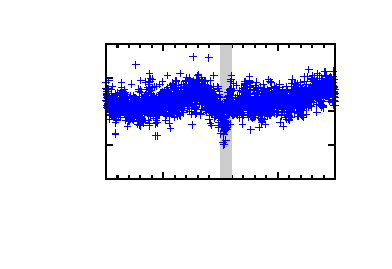
\includegraphics{/home/rik/workspace/ASL_student_project/Repositories/report-fork/Report/images/windazihour}}%
    \gplfronttext
  \end{picture}%
\endgroup

\label{fig:wind_azi_hour}}
\qquad
\subfloat[][{Wind speed $[ \si{\metre\per\second} ]$ from \formattime{5}{30}{0} to \formattime{5}{33}{0}  }]{
% GNUPLOT: LaTeX picture with Postscript
\begingroup
  \makeatletter
  \providecommand\color[2][]{%
    \GenericError{(gnuplot) \space\space\space\@spaces}{%
      Package color not loaded in conjunction with
      terminal option `colourtext'%
    }{See the gnuplot documentation for explanation.%
    }{Either use 'blacktext' in gnuplot or load the package
      color.sty in LaTeX.}%
    \renewcommand\color[2][]{}%
  }%
  \providecommand\includegraphics[2][]{%
    \GenericError{(gnuplot) \space\space\space\@spaces}{%
      Package graphicx or graphics not loaded%
    }{See the gnuplot documentation for explanation.%
    }{The gnuplot epslatex terminal needs graphicx.sty or graphics.sty.}%
    \renewcommand\includegraphics[2][]{}%
  }%
  \providecommand\rotatebox[2]{#2}%
  \@ifundefined{ifGPcolor}{%
    \newif\ifGPcolor
    \GPcolortrue
  }{}%
  \@ifundefined{ifGPblacktext}{%
    \newif\ifGPblacktext
    \GPblacktextfalse
  }{}%
  % define a \g@addto@macro without @ in the name:
  \let\gplgaddtomacro\g@addto@macro
  % define empty templates for all commands taking text:
  \gdef\gplbacktext{}%
  \gdef\gplfronttext{}%
  \makeatother
  \ifGPblacktext
    % no textcolor at all
    \def\colorrgb#1{}%
    \def\colorgray#1{}%
  \else
    % gray or color?
    \ifGPcolor
      \def\colorrgb#1{\color[rgb]{#1}}%
      \def\colorgray#1{\color[gray]{#1}}%
      \expandafter\def\csname LTw\endcsname{\color{white}}%
      \expandafter\def\csname LTb\endcsname{\color{black}}%
      \expandafter\def\csname LTa\endcsname{\color{black}}%
      \expandafter\def\csname LT0\endcsname{\color[rgb]{1,0,0}}%
      \expandafter\def\csname LT1\endcsname{\color[rgb]{0,1,0}}%
      \expandafter\def\csname LT2\endcsname{\color[rgb]{0,0,1}}%
      \expandafter\def\csname LT3\endcsname{\color[rgb]{1,0,1}}%
      \expandafter\def\csname LT4\endcsname{\color[rgb]{0,1,1}}%
      \expandafter\def\csname LT5\endcsname{\color[rgb]{1,1,0}}%
      \expandafter\def\csname LT6\endcsname{\color[rgb]{0,0,0}}%
      \expandafter\def\csname LT7\endcsname{\color[rgb]{1,0.3,0}}%
      \expandafter\def\csname LT8\endcsname{\color[rgb]{0.5,0.5,0.5}}%
    \else
      % gray
      \def\colorrgb#1{\color{black}}%
      \def\colorgray#1{\color[gray]{#1}}%
      \expandafter\def\csname LTw\endcsname{\color{white}}%
      \expandafter\def\csname LTb\endcsname{\color{black}}%
      \expandafter\def\csname LTa\endcsname{\color{black}}%
      \expandafter\def\csname LT0\endcsname{\color{black}}%
      \expandafter\def\csname LT1\endcsname{\color{black}}%
      \expandafter\def\csname LT2\endcsname{\color{black}}%
      \expandafter\def\csname LT3\endcsname{\color{black}}%
      \expandafter\def\csname LT4\endcsname{\color{black}}%
      \expandafter\def\csname LT5\endcsname{\color{black}}%
      \expandafter\def\csname LT6\endcsname{\color{black}}%
      \expandafter\def\csname LT7\endcsname{\color{black}}%
      \expandafter\def\csname LT8\endcsname{\color{black}}%
    \fi
  \fi
  \setlength{\unitlength}{0.0500bp}%
  \begin{picture}(3454.00,1700.00)%
    \gplgaddtomacro\gplbacktext{%
      \csname LTb\endcsname%
      \put(594,484){\makebox(0,0)[r]{\strut{} 0}}%
      \put(594,643){\makebox(0,0)[r]{\strut{} 2}}%
      \put(594,801){\makebox(0,0)[r]{\strut{} 4}}%
      \put(594,960){\makebox(0,0)[r]{\strut{} 6}}%
      \put(594,1118){\makebox(0,0)[r]{\strut{} 8}}%
      \put(594,1277){\makebox(0,0)[r]{\strut{} 10}}%
      \put(594,1435){\makebox(0,0)[r]{\strut{} 12}}%
      \put(726,264){\makebox(0,0){\strut{}30}}%
      \put(1503,264){\makebox(0,0){\strut{}31}}%
      \put(2280,264){\makebox(0,0){\strut{}32}}%
      \put(3057,264){\makebox(0,0){\strut{}33}}%
      \put(1891,154){\makebox(0,0){\strut{}time $[\si{\minute}]$}}%
    }%
    \gplgaddtomacro\gplfronttext{%
    }%
    \gplbacktext
    \put(0,0){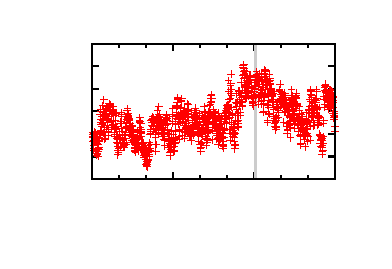
\includegraphics{/home/rik/workspace/ASL_student_project/Repositories/report-fork/Presentation/LaTeX_Template/images/windminute}}%
    \gplfronttext
  \end{picture}%
\endgroup

\label{fig:wind_speed_minutes}}
\subfloat[][{Wind azimuth $[ \si{\degree} ]$ from \formattime{5}{30}{0} to \formattime{5}{33}{0}  }]{
% GNUPLOT: LaTeX picture with Postscript
\begingroup
  \makeatletter
  \providecommand\color[2][]{%
    \GenericError{(gnuplot) \space\space\space\@spaces}{%
      Package color not loaded in conjunction with
      terminal option `colourtext'%
    }{See the gnuplot documentation for explanation.%
    }{Either use 'blacktext' in gnuplot or load the package
      color.sty in LaTeX.}%
    \renewcommand\color[2][]{}%
  }%
  \providecommand\includegraphics[2][]{%
    \GenericError{(gnuplot) \space\space\space\@spaces}{%
      Package graphicx or graphics not loaded%
    }{See the gnuplot documentation for explanation.%
    }{The gnuplot epslatex terminal needs graphicx.sty or graphics.sty.}%
    \renewcommand\includegraphics[2][]{}%
  }%
  \providecommand\rotatebox[2]{#2}%
  \@ifundefined{ifGPcolor}{%
    \newif\ifGPcolor
    \GPcolortrue
  }{}%
  \@ifundefined{ifGPblacktext}{%
    \newif\ifGPblacktext
    \GPblacktextfalse
  }{}%
  % define a \g@addto@macro without @ in the name:
  \let\gplgaddtomacro\g@addto@macro
  % define empty templates for all commands taking text:
  \gdef\gplbacktext{}%
  \gdef\gplfronttext{}%
  \makeatother
  \ifGPblacktext
    % no textcolor at all
    \def\colorrgb#1{}%
    \def\colorgray#1{}%
  \else
    % gray or color?
    \ifGPcolor
      \def\colorrgb#1{\color[rgb]{#1}}%
      \def\colorgray#1{\color[gray]{#1}}%
      \expandafter\def\csname LTw\endcsname{\color{white}}%
      \expandafter\def\csname LTb\endcsname{\color{black}}%
      \expandafter\def\csname LTa\endcsname{\color{black}}%
      \expandafter\def\csname LT0\endcsname{\color[rgb]{1,0,0}}%
      \expandafter\def\csname LT1\endcsname{\color[rgb]{0,1,0}}%
      \expandafter\def\csname LT2\endcsname{\color[rgb]{0,0,1}}%
      \expandafter\def\csname LT3\endcsname{\color[rgb]{1,0,1}}%
      \expandafter\def\csname LT4\endcsname{\color[rgb]{0,1,1}}%
      \expandafter\def\csname LT5\endcsname{\color[rgb]{1,1,0}}%
      \expandafter\def\csname LT6\endcsname{\color[rgb]{0,0,0}}%
      \expandafter\def\csname LT7\endcsname{\color[rgb]{1,0.3,0}}%
      \expandafter\def\csname LT8\endcsname{\color[rgb]{0.5,0.5,0.5}}%
    \else
      % gray
      \def\colorrgb#1{\color{black}}%
      \def\colorgray#1{\color[gray]{#1}}%
      \expandafter\def\csname LTw\endcsname{\color{white}}%
      \expandafter\def\csname LTb\endcsname{\color{black}}%
      \expandafter\def\csname LTa\endcsname{\color{black}}%
      \expandafter\def\csname LT0\endcsname{\color{black}}%
      \expandafter\def\csname LT1\endcsname{\color{black}}%
      \expandafter\def\csname LT2\endcsname{\color{black}}%
      \expandafter\def\csname LT3\endcsname{\color{black}}%
      \expandafter\def\csname LT4\endcsname{\color{black}}%
      \expandafter\def\csname LT5\endcsname{\color{black}}%
      \expandafter\def\csname LT6\endcsname{\color{black}}%
      \expandafter\def\csname LT7\endcsname{\color{black}}%
      \expandafter\def\csname LT8\endcsname{\color{black}}%
    \fi
  \fi
  \setlength{\unitlength}{0.0500bp}%
  \begin{picture}(3454.00,2266.00)%
    \gplgaddtomacro\gplbacktext{%
      \csname LTb\endcsname%
      \put(726,704){\makebox(0,0)[r]{\strut{} 0}}%
      \put(726,1028){\makebox(0,0)[r]{\strut{} 45}}%
      \put(726,1353){\makebox(0,0)[r]{\strut{} 90}}%
      \put(726,1677){\makebox(0,0)[r]{\strut{} 135}}%
      \put(726,2001){\makebox(0,0)[r]{\strut{} 180}}%
      \put(858,484){\makebox(0,0){\strut{}30}}%
      \put(1591,484){\makebox(0,0){\strut{}31}}%
      \put(2324,484){\makebox(0,0){\strut{}32}}%
      \put(3057,484){\makebox(0,0){\strut{}33}}%
      \put(1957,154){\makebox(0,0){\strut{}time $[\si{\minute}]$}}%
    }%
    \gplgaddtomacro\gplfronttext{%
    }%
    \gplbacktext
    \put(0,0){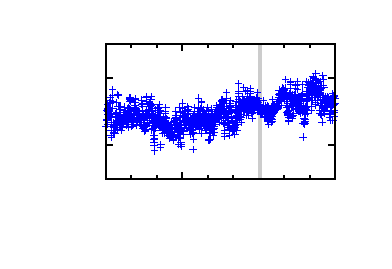
\includegraphics{/home/rik/workspace/ASL_student_project/Repositories/report-fork/Report/images/windaziminute}}%
    \gplfronttext
  \end{picture}%
\endgroup

\label{fig:wind_azi_minutes}}
\caption[Wind observations]{Wind observations. The data is gathered using an anemometer $2.76 \si{\metre}$ above ground in an open field in California, USA. More information and measurement data can be found in Google's open source data collection \cite{www:googleosb,www:googleheliostat}.}
\label{fig:wind_observations}
\end{figure}


In the bottom picture \subref{fig:wind_speed_minutes} one can detect a wind gust at \formattime{5}{32}{0}. The wind velocity suddenly reaches a peak of $10 \si{\metre\per\second}$ after averaging around $5 \si{\metre\per\second}$. 

However, the MAV position control action takes place in a even smaller time interval. For visualization a $3 \si{\second}$ interval has been highlighted with a vertical grey line in figure \ref{fig:wind_observations} \subref{fig:wind_speed_minutes} and \subref{fig:wind_azi_minutes}. 

Within this small time window the wind field can be modeled as a stationary stochastic process. The wind speed vector is characterised by a constant mean and variance.

\begin{align}
\E[\mathbf{w}(t)] &= \mean{\mathbf{w}} \\
\Var[\mathbf{w}(t)] &= \E\left[\left(\mathbf{w}(t)-\mean{\mathbf{w}} \right) \left(\mathbf{w}(t)-\mean{\mathbf{w}} \right)^T \right]  =\mathbf{ \Sigma }
\end{align}

Thus the differential equation governing the wind field is
\begin{align}
\d{\mathbf{w}(t)} &= \mathbf{ \Sigma } \d{\mathbf{W}(t)} \\
\mathbf{w}(0) &= \mean{\mathbf{w}}
\end{align}
where $\mathbf{W}(t)$ is standard Brownian motion.

A more convenient way is to state the dynamics as a discrete-time state space systems.
\begin{align}
\mathbf{w}(k+1) &= \mathbf{w}(k) + \mathbf{Q} \boldsymbol{\varepsilon}(k) \\ 
{\varepsilon}_i (k) &\sim \mathcal{N}(0,1) & \forall i \in \{ x,y,z \}
\label{eq:wind_state_space}
\end{align}


\subsection{Wind Forces}
Wind affects the MAV dynamics in two ways. On one hand it causes pressure on the multirotor surface opposed to the wind field. We call this load area drag $\mathbf{F}_A$. On the other hand the wind field influences the total rotor drag. We name this load drag force $\mathbf{F}_D$.

Schiano and others examined the effects of area drag on a Parrot AR Drone 2.0 (quadrotor) without polystyrene casing \cite{Schiano2014,www:parrot}. This MAV is a little smaller than the AscTec Firefly but the results are qualitatively comparable. They described area drag according to Rayleigh equations.

\begin{align}
\mathbf{F}_A = \frac{1}{2} C_A \rho \norm{\mathbf{w}}_2 \mathbf{w}  \label{eq:area_drag}
\end{align}
with
\begin{align*}
C_A&: & \text{area drag coefficient} \\
\rho&: &\text{air density} \\
\mathbf{w}&: &\text{wind speed}.
\end{align*}

In wind tunnel experiments they measured the forces on the switched off MAV for different angles of attack. They concluded that the drag coefficient is mainly a function of heading towards the wind. The worst case (largest force) equaled to $\psi = 90 \si{\degree}$, when the processor housing is exposed with the long side and thus the largest area towards the wind. 

Following rotor blade theory, the drag force is given as in equation \ref{eq:drag_force}.
\begin{align}
\mathbf{F}_D&= \sum_{i=1}^6 \omega_i \cdot  C_D \cdot _B\mathbf{\mathbf{w}}^\perp
\end{align}

Using the worst case area drag coefficient $C_A = 0.02$ from Schianos experiments and the rotor drag coefficent $C_D = \num{6.84 e-5}$ for the Firefly we simulate the resulting forces. Figure \ref{fig:area_vs_rotor_drag} shows the area and the rotor drag at different wind speeds and a hovering Firefly.    

\begin{figure} 
\centering 
% This file was created by matlab2tikz.
% Minimal pgfplots version: 1.3
%
%The latest updates can be retrieved from
%  http://www.mathworks.com/matlabcentral/fileexchange/22022-matlab2tikz
%where you can also make suggestions and rate matlab2tikz.
%
\definecolor{mycolor1}{rgb}{0.00000,0.44700,0.74100}%
\definecolor{mycolor2}{rgb}{0.85000,0.32500,0.09800}%
%
\begin{tikzpicture}

\begin{axis}[%
width=0.95092\figurewidth,
height=\figureheight,
at={(0\figurewidth,0\figureheight)},
scale only axis,
xmin=0,
xmax=20,
xlabel={Wind velocity $[\si{\metre\per\second}]$},
ymin=0,
ymax=6,
ytick={0, 1, 2, 3, 4, 5},
ylabel={Drag force [\si{\newton}]},
legend style={legend cell align=left,align=left,draw=white!15!black}
]
\addplot [color=mycolor1,solid]
  table[row sep=crcr]{%
0	0\\
0.02002002002002	4.90981471962453e-06\\
0.04004004004004	1.96392588784981e-05\\
0.0600600600600601	4.41883324766208e-05\\
0.0800800800800801	7.85570355139925e-05\\
0.1001001001001	0.000122745367990613\\
0.12012012012012	0.000176753329906483\\
0.14014014014014	0.000240580921261602\\
0.16016016016016	0.00031422814205597\\
0.18018018018018	0.000397694992289587\\
0.2002002002002	0.000490981471962453\\
0.22022022022022	0.000594087581074568\\
0.24024024024024	0.000707013319625932\\
0.26026026026026	0.000829758687616546\\
0.28028028028028	0.000962323685046408\\
0.3003003003003	0.00110470831191552\\
0.32032032032032	0.00125691256822388\\
0.34034034034034	0.00141893645397149\\
0.36036036036036	0.00159077996915835\\
0.38038038038038	0.00177244311378446\\
0.4004004004004	0.00196392588784981\\
0.42042042042042	0.00216522829135442\\
0.44044044044044	0.00237635032429827\\
0.46046046046046	0.00259729198668138\\
0.48048048048048	0.00282805327850373\\
0.500500500500501	0.00306863419976533\\
0.520520520520521	0.00331903475046618\\
0.540540540540541	0.00357925493060628\\
0.560560560560561	0.00384929474018563\\
0.580580580580581	0.00412915417920423\\
0.600600600600601	0.00441883324766208\\
0.620620620620621	0.00471833194555917\\
0.640640640640641	0.00502765027289552\\
0.660660660660661	0.00534678822967111\\
0.680680680680681	0.00567574581588596\\
0.700700700700701	0.00601452303154005\\
0.720720720720721	0.00636311987663339\\
0.740740740740741	0.00672153635116598\\
0.760760760760761	0.00708977245513782\\
0.780780780780781	0.00746782818854891\\
0.800800800800801	0.00785570355139925\\
0.820820820820821	0.00825339854368884\\
0.840840840840841	0.00866091316541767\\
0.860860860860861	0.00907824741658575\\
0.880880880880881	0.00950540129719309\\
0.900900900900901	0.00994237480723967\\
0.920920920920921	0.0103891679467255\\
0.940940940940941	0.0108457807156506\\
0.960960960960961	0.0113122131140149\\
0.980980980980981	0.0117884651418185\\
1.001001001001	0.0122745367990613\\
1.02102102102102	0.0127704280857434\\
1.04104104104104	0.0132761390018647\\
1.06106106106106	0.0137916695474253\\
1.08108108108108	0.0143170197224251\\
1.1011011011011	0.0148521895268642\\
1.12112112112112	0.0153971789607425\\
1.14114114114114	0.0159519880240601\\
1.16116116116116	0.0165166167168169\\
1.18118118118118	0.017091065039013\\
1.2012012012012	0.0176753329906483\\
1.22122122122122	0.0182694205717229\\
1.24124124124124	0.0188733277822367\\
1.26126126126126	0.0194870546221898\\
1.28128128128128	0.0201106010915821\\
1.3013013013013	0.0207439671904136\\
1.32132132132132	0.0213871529186845\\
1.34134134134134	0.0220401582763945\\
1.36136136136136	0.0227029832635438\\
1.38138138138138	0.0233756278801324\\
1.4014014014014	0.0240580921261602\\
1.42142142142142	0.0247503760016273\\
1.44144144144144	0.0254524795065336\\
1.46146146146146	0.0261644026408791\\
1.48148148148148	0.0268861454046639\\
1.5015015015015	0.027617707797888\\
1.52152152152152	0.0283590898205513\\
1.54154154154154	0.0291102914726538\\
1.56156156156156	0.0298713127541956\\
1.58158158158158	0.0306421536651767\\
1.6016016016016	0.031422814205597\\
1.62162162162162	0.0322132943754565\\
1.64164164164164	0.0330135941747553\\
1.66166166166166	0.0338237136034934\\
1.68168168168168	0.0346436526616707\\
1.7017017017017	0.0354734113492872\\
1.72172172172172	0.036312989666343\\
1.74174174174174	0.0371623876128381\\
1.76176176176176	0.0380216051887724\\
1.78178178178178	0.0388906423941459\\
1.8018018018018	0.0397694992289587\\
1.82182182182182	0.0406581756932107\\
1.84184184184184	0.041556671786902\\
1.86186186186186	0.0424649875100326\\
1.88188188188188	0.0433831228626023\\
1.9019019019019	0.0443110778446114\\
1.92192192192192	0.0452488524560597\\
1.94194194194194	0.0461964466969472\\
1.96196196196196	0.047153860567274\\
1.98198198198198	0.04812109406704\\
2.002002002002	0.0490981471962453\\
2.02202202202202	0.0500850199548898\\
2.04204204204204	0.0510817123429736\\
2.06206206206206	0.0520882243604966\\
2.08208208208208	0.0531045560074589\\
2.1021021021021	0.0541307072838604\\
2.12212212212212	0.0551666781897012\\
2.14214214214214	0.0562124687249812\\
2.16216216216216	0.0572680788897005\\
2.18218218218218	0.058333508683859\\
2.2022022022022	0.0594087581074568\\
2.22222222222222	0.0604938271604938\\
2.24224224224224	0.0615887158429701\\
2.26226226226226	0.0626934241548856\\
2.28228228228228	0.0638079520962404\\
2.3023023023023	0.0649322996670344\\
2.32232232232232	0.0660664668672677\\
2.34234234234234	0.0672104536969402\\
2.36236236236236	0.068364260156052\\
2.38238238238238	0.069527886244603\\
2.4024024024024	0.0707013319625932\\
2.42242242242242	0.0718845973100227\\
2.44244244244244	0.0730776822868915\\
2.46246246246246	0.0742805868931995\\
2.48248248248248	0.0754933111289468\\
2.5025025025025	0.0767158549941333\\
2.52252252252252	0.077948218488759\\
2.54254254254254	0.079190401612824\\
2.56256256256256	0.0804424043663283\\
2.58258258258258	0.0817042267492718\\
2.6026026026026	0.0829758687616546\\
2.62262262262262	0.0842573304034765\\
2.64264264264264	0.0855486116747378\\
2.66266266266266	0.0868497125754383\\
2.68268268268268	0.088160633105578\\
2.7027027027027	0.089481373265157\\
2.72272272272272	0.0908119330541753\\
2.74274274274274	0.0921523124726328\\
2.76276276276276	0.0935025115205295\\
2.78278278278278	0.0948625301978655\\
2.8028028028028	0.0962323685046408\\
2.82282282282282	0.0976120264408553\\
2.84284284284284	0.099001504006509\\
2.86286286286286	0.100400801201602\\
2.88288288288288	0.101809918026134\\
2.9029029029029	0.103228854480106\\
2.92292292292292	0.104657610563516\\
2.94294294294294	0.106096186276366\\
2.96296296296296	0.107544581618656\\
2.98298298298298	0.109002796590384\\
3.003003003003	0.110470831191552\\
3.02302302302302	0.111948685422159\\
3.04304304304304	0.113436359282205\\
3.06306306306306	0.114933852771691\\
3.08308308308308	0.116441165890615\\
3.1031031031031	0.117958298638979\\
3.12312312312312	0.119485251016783\\
3.14314314314314	0.121022023024025\\
3.16316316316316	0.122568614660707\\
3.18318318318318	0.124125025926828\\
3.2032032032032	0.125691256822388\\
3.22322322322322	0.127267307347387\\
3.24324324324324	0.128853177501826\\
3.26326326326326	0.130448867285704\\
3.28328328328328	0.132054376699021\\
3.3033033033033	0.133669705741778\\
3.32332332332332	0.135294854413974\\
3.34334334334334	0.136929822715609\\
3.36336336336336	0.138574610646683\\
3.38338338338338	0.140229218207196\\
3.4034034034034	0.141893645397149\\
3.42342342342342	0.143567892216541\\
3.44344344344344	0.145251958665372\\
3.46346346346346	0.146945844743643\\
3.48348348348348	0.148649550451352\\
3.5035035035035	0.150363075788501\\
3.52352352352352	0.152086420755089\\
3.54354354354354	0.153819585351117\\
3.56356356356356	0.155562569576584\\
3.58358358358358	0.15731537343149\\
3.6036036036036	0.159077996915835\\
3.62362362362362	0.160850440029619\\
3.64364364364364	0.162632702772843\\
3.66366366366366	0.164424785145506\\
3.68368368368368	0.166226687147608\\
3.7037037037037	0.16803840877915\\
3.72372372372372	0.16985995004013\\
3.74374374374374	0.17169131093055\\
3.76376376376376	0.173532491450409\\
3.78378378378378	0.175383491599708\\
3.8038038038038	0.177244311378446\\
3.82382382382382	0.179114950786622\\
3.84384384384384	0.180995409824239\\
3.86386386386386	0.182885688491294\\
3.88388388388388	0.184785786787789\\
3.9039039039039	0.186695704713723\\
3.92392392392392	0.188615442269096\\
3.94394394394394	0.190544999453908\\
3.96396396396396	0.19248437626816\\
3.98398398398398	0.194433572711851\\
4.004004004004	0.196392588784981\\
4.02402402402402	0.198361424487551\\
4.04404404404404	0.200340079819559\\
4.06406406406406	0.202328554781007\\
4.08408408408408	0.204326849371894\\
4.1041041041041	0.206334963592221\\
4.12412412412412	0.208352897441987\\
4.14414414414414	0.210380650921192\\
4.16416416416416	0.212418224029836\\
4.18418418418418	0.214465616767919\\
4.2042042042042	0.216522829135442\\
4.22422422422422	0.218589861132404\\
4.24424424424424	0.220666712758805\\
4.26426426426426	0.222753384014645\\
4.28428428428428	0.224849874899925\\
4.3043043043043	0.226956185414644\\
4.32432432432432	0.229072315558802\\
4.34434434434434	0.2311982653324\\
4.36436436436436	0.233334034735436\\
4.38438438438438	0.235479623767912\\
4.4044044044044	0.237635032429827\\
4.42442442442442	0.239800260721182\\
4.44444444444444	0.241975308641975\\
4.46446446446446	0.244160176192208\\
4.48448448448448	0.24635486337188\\
4.5045045045045	0.248559370180992\\
4.52452452452452	0.250773696619542\\
4.54454454454454	0.252997842687532\\
4.56456456456456	0.255231808384962\\
4.58458458458458	0.25747559371183\\
4.6046046046046	0.259729198668138\\
4.62462462462462	0.261992623253885\\
4.64464464464464	0.264265867469071\\
4.66466466466466	0.266548931313696\\
4.68468468468468	0.268841814787761\\
4.7047047047047	0.271144517891265\\
4.72472472472472	0.273457040624208\\
4.74474474474474	0.27577938298659\\
4.76476476476476	0.278111544978412\\
4.78478478478478	0.280453526599673\\
4.8048048048048	0.282805327850373\\
4.82482482482482	0.285166948730512\\
4.84484484484484	0.287538389240091\\
4.86486486486486	0.289919649379109\\
4.88488488488488	0.292310729147566\\
4.9049049049049	0.294711628545462\\
4.92492492492492	0.297122347572798\\
4.94494494494494	0.299542886229573\\
4.96496496496496	0.301973244515787\\
4.98498498498498	0.30441342243144\\
5.00500500500501	0.306863419976533\\
5.02502502502503	0.309323237151065\\
5.04504504504505	0.311792873955036\\
5.06506506506507	0.314272330388447\\
5.08508508508509	0.316761606451296\\
5.10510510510511	0.319260702143585\\
5.12512512512513	0.321769617465313\\
5.14514514514515	0.324288352416481\\
5.16516516516517	0.326816906997087\\
5.18518518518519	0.329355281207133\\
5.20520520520521	0.331903475046618\\
5.22522522522523	0.334461488515543\\
5.24524524524525	0.337029321613906\\
5.26526526526527	0.339606974341709\\
5.28528528528529	0.342194446698951\\
5.30530530530531	0.344791738685633\\
5.32532532532533	0.347398850301753\\
5.34534534534535	0.350015781547313\\
5.36536536536537	0.352642532422312\\
5.38538538538539	0.355279102926751\\
5.40540540540541	0.357925493060628\\
5.42542542542543	0.360581702823945\\
5.44544544544545	0.363247732216701\\
5.46546546546547	0.365923581238897\\
5.48548548548549	0.368609249890531\\
5.50550550550551	0.371304738171605\\
5.52552552552553	0.374010046082118\\
5.54554554554555	0.37672517362207\\
5.56556556556557	0.379450120791462\\
5.58558558558559	0.382184887590293\\
5.60560560560561	0.384929474018563\\
5.62562562562563	0.387683880076272\\
5.64564564564565	0.390448105763421\\
5.66566566566567	0.393222151080009\\
5.68568568568569	0.396006016026036\\
5.70570570570571	0.398799700601502\\
5.72572572572573	0.401603204806408\\
5.74574574574575	0.404416528640753\\
5.76576576576577	0.407239672104537\\
5.78578578578579	0.41007263519776\\
5.80580580580581	0.412915417920423\\
5.82582582582583	0.415768020272525\\
5.84584584584585	0.418630442254066\\
5.86586586586587	0.421502683865046\\
5.88588588588589	0.424384745105466\\
5.90590590590591	0.427276625975325\\
5.92592592592593	0.430178326474623\\
5.94594594594595	0.43308984660336\\
5.96596596596597	0.436011186361537\\
5.98598598598599	0.438942345749153\\
6.00600600600601	0.441883324766208\\
6.02602602602603	0.444834123412702\\
6.04604604604605	0.447794741688636\\
6.06606606606607	0.450765179594008\\
6.08608608608609	0.45374543712882\\
6.10610610610611	0.456735514293072\\
6.12612612612613	0.459735411086762\\
6.14614614614615	0.462745127509892\\
6.16616616616617	0.465764663562461\\
6.18618618618619	0.46879401924447\\
6.20620620620621	0.471833194555917\\
6.22622622622623	0.474882189496804\\
6.24624624624625	0.47794100406713\\
6.26626626626627	0.481009638266896\\
6.28628628628629	0.4840880920961\\
6.30630630630631	0.487176365554744\\
6.32632632632633	0.490274458642827\\
6.34634634634635	0.493382371360349\\
6.36636636636637	0.496500103707311\\
6.38638638638639	0.499627655683712\\
6.40640640640641	0.502765027289552\\
6.42642642642643	0.505912218524831\\
6.44644644644645	0.50906922938955\\
6.46646646646647	0.512236059883708\\
6.48648648648649	0.515412710007305\\
6.50650650650651	0.518599179760341\\
6.52652652652653	0.521795469142816\\
6.54654654654655	0.525001578154731\\
6.56656656656657	0.528217506796085\\
6.58658658658659	0.531443255066879\\
6.60660660660661	0.534678822967111\\
6.62662662662663	0.537924210496783\\
6.64664664664665	0.541179417655894\\
6.66666666666667	0.544444444444445\\
6.68668668668669	0.547719290862434\\
6.70670670670671	0.551003956909863\\
6.72672672672673	0.554298442586731\\
6.74674674674675	0.557602747893038\\
6.76676676676677	0.560916872828785\\
6.78678678678679	0.564240817393971\\
6.80680680680681	0.567574581588596\\
6.82682682682683	0.57091816541266\\
6.84684684684685	0.574271568866163\\
6.86686686686687	0.577634791949106\\
6.88688688688689	0.581007834661488\\
6.90690690690691	0.58439069700331\\
6.92692692692693	0.58778337897457\\
6.94694694694695	0.59118588057527\\
6.96696696696697	0.594598201805409\\
6.98698698698699	0.598020342664987\\
7.00700700700701	0.601452303154005\\
7.02702702702703	0.604894083272462\\
7.04704704704705	0.608345683020358\\
7.06706706706707	0.611807102397693\\
7.08708708708709	0.615278341404468\\
7.10710710710711	0.618759400040681\\
7.12712712712713	0.622250278306334\\
7.14714714714715	0.625750976201427\\
7.16716716716717	0.629261493725958\\
7.18718718718719	0.632781830879929\\
7.20720720720721	0.636311987663339\\
7.22722722722723	0.639851964076188\\
7.24724724724725	0.643401760118477\\
7.26726726726727	0.646961375790205\\
7.28728728728729	0.650530811091372\\
7.30730730730731	0.654110066021978\\
7.32732732732733	0.657699140582024\\
7.34734734734735	0.661298034771508\\
7.36736736736737	0.664906748590432\\
7.38738738738739	0.668525282038796\\
7.40740740740741	0.672153635116598\\
7.42742742742743	0.67579180782384\\
7.44744744744745	0.679439800160521\\
7.46746746746747	0.683097612126641\\
7.48748748748749	0.686765243722201\\
7.50750750750751	0.690442694947199\\
7.52752752752753	0.694129965801638\\
7.54754754754755	0.697827056285515\\
7.56756756756757	0.701533966398831\\
7.58758758758759	0.705250696141587\\
7.60760760760761	0.708977245513782\\
7.62762762762763	0.712713614515416\\
7.64764764764765	0.71645980314649\\
7.66766766766767	0.720215811407003\\
7.68768768768769	0.723981639296955\\
7.70770770770771	0.727757286816346\\
7.72772772772773	0.731542753965176\\
7.74774774774775	0.735338040743446\\
7.76776776776777	0.739143147151155\\
7.78778778778779	0.742958073188303\\
7.80780780780781	0.746782818854891\\
7.82782782782783	0.750617384150918\\
7.84784784784785	0.754461769076384\\
7.86786786786787	0.758315973631289\\
7.88788788788789	0.762179997815634\\
7.90790790790791	0.766053841629417\\
7.92792792792793	0.76993750507264\\
7.94794794794795	0.773830988145302\\
7.96796796796797	0.777734290847404\\
7.98798798798799	0.781647413178945\\
8.00800800800801	0.785570355139925\\
8.02802802802803	0.789503116730344\\
8.04804804804805	0.793445697950203\\
8.06806806806807	0.7973980987995\\
8.08808808808809	0.801360319278237\\
8.10810810810811	0.805332359386414\\
8.12812812812813	0.809314219124029\\
8.14814814814815	0.813305898491084\\
8.16816816816817	0.817307397487578\\
8.18818818818819	0.821318716113511\\
8.20820820820821	0.825339854368884\\
8.22822822822823	0.829370812253695\\
8.24824824824825	0.833411589767946\\
8.26826826826827	0.837462186911636\\
8.28828828828829	0.841522603684766\\
8.30830830830831	0.845592840087335\\
8.32832832832833	0.849672896119343\\
8.34834834834835	0.85376277178079\\
8.36836836836837	0.857862467071676\\
8.38838838838839	0.861971981992002\\
8.40840840840841	0.866091316541767\\
8.42842842842843	0.870220470720971\\
8.44844844844845	0.874359444529615\\
8.46846846846847	0.878508237967698\\
8.48848848848849	0.88266685103522\\
8.50850850850851	0.886835283732181\\
8.52852852852853	0.891013536058581\\
8.54854854854855	0.895201608014421\\
8.56856856856857	0.8993994995997\\
8.58858858858859	0.903607210814418\\
8.60860860860861	0.907824741658576\\
8.62862862862863	0.912052092132172\\
8.64864864864865	0.916289262235208\\
8.66866866866867	0.920536251967683\\
8.68868868868869	0.924793061329598\\
8.70870870870871	0.929059690320952\\
8.72872872872873	0.933336138941745\\
8.74874874874875	0.937622407191977\\
8.76876876876877	0.941918495071648\\
8.78878878878879	0.946224402580759\\
8.80880880880881	0.950540129719309\\
8.82882882882883	0.954865676487298\\
8.84884884884885	0.959201042884727\\
8.86886886886887	0.963546228911594\\
8.88888888888889	0.967901234567901\\
8.90890890890891	0.972266059853648\\
8.92892892892893	0.976640704768833\\
8.94894894894895	0.981025169313458\\
8.96896896896897	0.985419453487522\\
8.98898898898899	0.989823557291025\\
9.00900900900901	0.994237480723967\\
9.02902902902903	0.998661223786349\\
9.04904904904905	1.00309478647817\\
9.06906906906907	1.00753816879943\\
9.08908908908909	1.01199137075013\\
9.10910910910911	1.01645439233027\\
9.12912912912913	1.02092723353985\\
9.14914914914915	1.02540989437886\\
9.16916916916917	1.02990237484732\\
9.18918918918919	1.03440467494522\\
9.20920920920921	1.03891679467255\\
9.22922922922923	1.04343873402932\\
9.24924924924925	1.04797049301554\\
9.26926926926927	1.05251207163119\\
9.28928928928929	1.05706346987628\\
9.30930930930931	1.06162468775081\\
9.32932932932933	1.06619572525478\\
9.34934934934935	1.07077658238819\\
9.36936936936937	1.07536725915104\\
9.38938938938939	1.07996775554333\\
9.40940940940941	1.08457807156506\\
9.42942942942943	1.08919820721623\\
9.44944944944945	1.09382816249683\\
9.46946946946947	1.09846793740688\\
9.48948948948949	1.10311753194636\\
9.50950950950951	1.10777694611528\\
9.52952952952953	1.11244617991365\\
9.54954954954955	1.11712523334145\\
9.56956956956957	1.12181410639869\\
9.58958958958959	1.12651279908537\\
9.60960960960961	1.13122131140149\\
9.62962962962963	1.13593964334705\\
9.64964964964965	1.14066779492205\\
9.66966966966967	1.14540576612649\\
9.68968968968969	1.15015355696036\\
9.70970970970971	1.15491116742368\\
9.72972972972973	1.15967859751644\\
9.74974974974975	1.16445584723863\\
9.76976976976977	1.16924291659026\\
9.78978978978979	1.17403980557134\\
9.80980980980981	1.17884651418185\\
9.82982982982983	1.1836630424218\\
9.84984984984985	1.18848939029119\\
9.86986986986987	1.19332555779002\\
9.88988988988989	1.19817154491829\\
9.90990990990991	1.203027351676\\
9.92992992992993	1.20789297806315\\
9.94994994994995	1.21276842407974\\
9.96996996996997	1.21765368972576\\
9.98998998998999	1.22254877500123\\
10.01001001001	1.22745367990613\\
10.03003003003	1.23236840444048\\
10.0500500500501	1.23729294860426\\
10.0700700700701	1.24222731239748\\
10.0900900900901	1.24717149582014\\
10.1101101101101	1.25212549887225\\
10.1301301301301	1.25708932155379\\
10.1501501501502	1.26206296386477\\
10.1701701701702	1.26704642580518\\
10.1901901901902	1.27203970737504\\
10.2102102102102	1.27704280857434\\
10.2302302302302	1.28205572940308\\
10.2502502502503	1.28707846986125\\
10.2702702702703	1.29211102994887\\
10.2902902902903	1.29715340966592\\
10.3103103103103	1.30220560901242\\
10.3303303303303	1.30726762798835\\
10.3503503503504	1.31233946659372\\
10.3703703703704	1.31742112482853\\
10.3903903903904	1.32251260269278\\
10.4104104104104	1.32761390018647\\
10.4304304304304	1.3327250173096\\
10.4504504504505	1.33784595406217\\
10.4704704704705	1.34297671044418\\
10.4904904904905	1.34811728645562\\
10.5105105105105	1.35326768209651\\
10.5305305305305	1.35842789736684\\
10.5505505505506	1.3635979322666\\
10.5705705705706	1.3687777867958\\
10.5905905905906	1.37396746095445\\
10.6106106106106	1.37916695474253\\
10.6306306306306	1.38437626816005\\
10.6506506506507	1.38959540120701\\
10.6706706706707	1.39482435388341\\
10.6906906906907	1.40006312618925\\
10.7107107107107	1.40531171812453\\
10.7307307307307	1.41057012968925\\
10.7507507507508	1.41583836088341\\
10.7707707707708	1.421116411707\\
10.7907907907908	1.42640428216004\\
10.8108108108108	1.43170197224251\\
10.8308308308308	1.43700948195443\\
10.8508508508509	1.44232681129578\\
10.8708708708709	1.44765396026657\\
10.8908908908909	1.4529909288668\\
10.9109109109109	1.45833771709648\\
10.9309309309309	1.46369432495559\\
10.950950950951	1.46906075244414\\
10.970970970971	1.47443699956212\\
10.990990990991	1.47982306630955\\
11.011011011011	1.48521895268642\\
11.031031031031	1.49062465869273\\
11.0510510510511	1.49604018432847\\
11.0710710710711	1.50146552959366\\
11.0910910910911	1.50690069448828\\
11.1111111111111	1.51234567901235\\
11.1311311311311	1.51780048316585\\
11.1511511511512	1.52326510694879\\
11.1711711711712	1.52873955036117\\
11.1911911911912	1.53422381340299\\
11.2112112112112	1.53971789607425\\
11.2312312312312	1.54522179837495\\
11.2512512512513	1.55073552030509\\
11.2712712712713	1.55625906186467\\
11.2912912912913	1.56179242305368\\
11.3113113113113	1.56733560387214\\
11.3313313313313	1.57288860432004\\
11.3513513513514	1.57845142439737\\
11.3713713713714	1.58402406410414\\
11.3913913913914	1.58960652344036\\
11.4114114114114	1.59519880240601\\
11.4314314314314	1.6008009010011\\
11.4514514514515	1.60641281922563\\
11.4714714714715	1.6120345570796\\
11.4914914914915	1.61766611456301\\
11.5115115115115	1.62330749167586\\
11.5315315315315	1.62895868841815\\
11.5515515515516	1.63461970478987\\
11.5715715715716	1.64029054079104\\
11.5915915915916	1.64597119642165\\
11.6116116116116	1.65166167168169\\
11.6316316316316	1.65736196657118\\
11.6516516516517	1.6630720810901\\
11.6716716716717	1.66879201523846\\
11.6916916916917	1.67452176901626\\
11.7117117117117	1.6802613424235\\
11.7317317317317	1.68601073546018\\
11.7517517517518	1.6917699481263\\
11.7717717717718	1.69753898042186\\
11.7917917917918	1.70331783234686\\
11.8118118118118	1.7091065039013\\
11.8318318318318	1.71490499508518\\
11.8518518518519	1.72071330589849\\
11.8718718718719	1.72653143634125\\
11.8918918918919	1.73235938641344\\
11.9119119119119	1.73819715611507\\
11.9319319319319	1.74404474544615\\
11.951951951952	1.74990215440666\\
11.971971971972	1.75576938299661\\
11.991991991992	1.761646431216\\
12.012012012012	1.76753329906483\\
12.032032032032	1.7734299865431\\
12.0520520520521	1.77933649365081\\
12.0720720720721	1.78525282038796\\
12.0920920920921	1.79117896675454\\
12.1121121121121	1.79711493275057\\
12.1321321321321	1.80306071837603\\
12.1521521521522	1.80901632363094\\
12.1721721721722	1.81498174851528\\
12.1921921921922	1.82095699302906\\
12.2122122122122	1.82694205717229\\
12.2322322322322	1.83293694094495\\
12.2522522522523	1.83894164434705\\
12.2722722722723	1.84495616737859\\
12.2922922922923	1.85098051003957\\
12.3123123123123	1.85701467232999\\
12.3323323323323	1.86305865424985\\
12.3523523523524	1.86911245579914\\
12.3723723723724	1.87517607697788\\
12.3923923923924	1.88124951778605\\
12.4124124124124	1.88733277822367\\
12.4324324324324	1.89342585829072\\
12.4524524524525	1.89952875798722\\
12.4724724724725	1.90564147731315\\
12.4924924924925	1.91176401626852\\
12.5125125125125	1.91789637485333\\
12.5325325325325	1.92403855306758\\
12.5525525525526	1.93019055091127\\
12.5725725725726	1.9363523683844\\
12.5925925925926	1.94252400548697\\
12.6126126126126	1.94870546221898\\
12.6326326326326	1.95489673858042\\
12.6526526526527	1.96109783457131\\
12.6726726726727	1.96730875019163\\
12.6926926926927	1.9735294854414\\
12.7127127127127	1.9797600403206\\
12.7327327327327	1.98600041482924\\
12.7527527527528	1.99225060896733\\
12.7727727727728	1.99851062273485\\
12.7927927927928	2.00478045613181\\
12.8128128128128	2.01106010915821\\
12.8328328328328	2.01734958181405\\
12.8528528528529	2.02364887409933\\
12.8728728728729	2.02995798601404\\
12.8928928928929	2.0362769175582\\
12.9129129129129	2.0426056687318\\
12.9329329329329	2.04894423953483\\
12.952952952953	2.05529262996731\\
12.972972972973	2.06165084002922\\
12.992992992993	2.06801886972057\\
13.013013013013	2.07439671904136\\
13.033033033033	2.0807843879916\\
13.0530530530531	2.08718187657127\\
13.0730730730731	2.09358918478038\\
13.0930930930931	2.10000631261893\\
13.1131131131131	2.10643326008691\\
13.1331331331331	2.11287002718434\\
13.1531531531532	2.11931661391121\\
13.1731731731732	2.12577302026752\\
13.1931931931932	2.13223924625326\\
13.2132132132132	2.13871529186845\\
13.2332332332332	2.14520115711307\\
13.2532532532533	2.15169684198713\\
13.2732732732733	2.15820234649064\\
13.2932932932933	2.16471767062358\\
13.3133133133133	2.17124281438596\\
13.3333333333333	2.17777777777778\\
13.3533533533534	2.18432256079904\\
13.3733733733734	2.19087716344974\\
13.3933933933934	2.19744158572987\\
13.4134134134134	2.20401582763945\\
13.4334334334334	2.21059988917847\\
13.4534534534535	2.21719377034692\\
13.4734734734735	2.22379747114482\\
13.4934934934935	2.23041099157215\\
13.5135135135135	2.23703433162893\\
13.5335335335335	2.24366749131514\\
13.5535535535536	2.25031047063079\\
13.5735735735736	2.25696326957588\\
13.5935935935936	2.26362588815041\\
13.6136136136136	2.27029832635438\\
13.6336336336336	2.27698058418779\\
13.6536536536537	2.28367266165064\\
13.6736736736737	2.29037455874293\\
13.6936936936937	2.29708627546465\\
13.7137137137137	2.30380781181582\\
13.7337337337337	2.31053916779643\\
13.7537537537538	2.31728034340647\\
13.7737737737738	2.32403133864595\\
13.7937937937938	2.33079215351488\\
13.8138138138138	2.33756278801324\\
13.8338338338338	2.34434324214104\\
13.8538538538539	2.35113351589828\\
13.8738738738739	2.35793360928496\\
13.8938938938939	2.36474352230108\\
13.9139139139139	2.37156325494664\\
13.9339339339339	2.37839280722164\\
13.953953953954	2.38523217912607\\
13.973973973974	2.39208137065995\\
13.993993993994	2.39894038182326\\
14.014014014014	2.40580921261602\\
14.034034034034	2.41268786303821\\
14.0540540540541	2.41957633308985\\
14.0740740740741	2.42647462277092\\
14.0940940940941	2.43338273208143\\
14.1141141141141	2.44030066102138\\
14.1341341341341	2.44722840959077\\
14.1541541541542	2.4541659777896\\
14.1741741741742	2.46111336561787\\
14.1941941941942	2.46807057307558\\
14.2142142142142	2.47503760016273\\
14.2342342342342	2.48201444687931\\
14.2542542542543	2.48900111322534\\
14.2742742742743	2.4959975992008\\
14.2942942942943	2.50300390480571\\
14.3143143143143	2.51002003004005\\
14.3343343343343	2.51704597490383\\
14.3543543543544	2.52408173939705\\
14.3743743743744	2.53112732351972\\
14.3943943943944	2.53818272727182\\
14.4144144144144	2.54524795065336\\
14.4344344344344	2.55232299366434\\
14.4544544544545	2.55940785630475\\
14.4744744744745	2.56650253857461\\
14.4944944944945	2.57360704047391\\
14.5145145145145	2.58072136200264\\
14.5345345345345	2.58784550316082\\
14.5545545545546	2.59497946394843\\
14.5745745745746	2.60212324436549\\
14.5945945945946	2.60927684441198\\
14.6146146146146	2.61644026408791\\
14.6346346346346	2.62361350339328\\
14.6546546546547	2.63079656232809\\
14.6746746746747	2.63798944089234\\
14.6946946946947	2.64519213908603\\
14.7147147147147	2.65240465690916\\
14.7347347347347	2.65962699436173\\
14.7547547547548	2.66685915144374\\
14.7747747747748	2.67410112815518\\
14.7947947947948	2.68135292449607\\
14.8148148148148	2.68861454046639\\
14.8348348348348	2.69588597606616\\
14.8548548548549	2.70316723129536\\
14.8748748748749	2.710458306154\\
14.8948948948949	2.71775920064208\\
14.9149149149149	2.7250699147596\\
14.9349349349349	2.73239044850656\\
14.954954954955	2.73972080188296\\
14.974974974975	2.7470609748888\\
14.994994994995	2.75441096752408\\
15.015015015015	2.7617707797888\\
15.035035035035	2.76914041168295\\
15.0550550550551	2.77651986320655\\
15.0750750750751	2.78390913435959\\
15.0950950950951	2.79130822514206\\
15.1151151151151	2.79871713555397\\
15.1351351351351	2.80613586559533\\
15.1551551551552	2.81356441526612\\
15.1751751751752	2.82100278456635\\
15.1951951951952	2.82845097349602\\
15.2152152152152	2.83590898205513\\
15.2352352352352	2.84337681024368\\
15.2552552552553	2.85085445806167\\
15.2752752752753	2.85834192550909\\
15.2952952952953	2.86583921258596\\
15.3153153153153	2.87334631929227\\
15.3353353353353	2.88086324562801\\
15.3553553553554	2.88838999159319\\
15.3753753753754	2.89592655718782\\
15.3953953953954	2.90347294241188\\
15.4154154154154	2.91102914726538\\
15.4354354354354	2.91859517174832\\
15.4554554554555	2.92617101586071\\
15.4754754754755	2.93375667960253\\
15.4954954954955	2.94135216297378\\
15.5155155155155	2.94895746597448\\
15.5355355355355	2.95657258860462\\
15.5555555555556	2.9641975308642\\
15.5755755755756	2.97183229275321\\
15.5955955955956	2.97947687427167\\
15.6156156156156	2.98713127541956\\
15.6356356356356	2.9947954961969\\
15.6556556556557	3.00246953660367\\
15.6756756756757	3.01015339663988\\
15.6956956956957	3.01784707630553\\
15.7157157157157	3.02555057560063\\
15.7357357357357	3.03326389452516\\
15.7557557557558	3.04098703307913\\
15.7757757757758	3.04871999126253\\
15.7957957957958	3.05646276907538\\
15.8158158158158	3.06421536651767\\
15.8358358358358	3.0719777835894\\
15.8558558558559	3.07975002029056\\
15.8758758758759	3.08753207662117\\
15.8958958958959	3.09532395258121\\
15.9159159159159	3.10312564817069\\
15.9359359359359	3.11093716338962\\
15.955955955956	3.11875849823798\\
15.975975975976	3.12658965271578\\
15.995995995996	3.13443062682302\\
16.016016016016	3.1422814205597\\
16.036036036036	3.15014203392582\\
16.0560560560561	3.15801246692138\\
16.0760760760761	3.16589271954637\\
16.0960960960961	3.17378279180081\\
16.1161161161161	3.18168268368469\\
16.1361361361361	3.189592395198\\
16.1561561561562	3.19751192634076\\
16.1761761761762	3.20544127711295\\
16.1961961961962	3.21338044751458\\
16.2162162162162	3.22132943754565\\
16.2362362362362	3.22928824720617\\
16.2562562562563	3.23725687649612\\
16.2762762762763	3.24523532541551\\
16.2962962962963	3.25322359396434\\
16.3163163163163	3.2612216821426\\
16.3363363363363	3.26922958995031\\
16.3563563563564	3.27724731738746\\
16.3763763763764	3.28527486445404\\
16.3963963963964	3.29331223115007\\
16.4164164164164	3.30135941747553\\
16.4364364364364	3.30941642343044\\
16.4564564564565	3.31748324901478\\
16.4764764764765	3.32555989422856\\
16.4964964964965	3.33364635907179\\
16.5165165165165	3.34174264354445\\
16.5365365365365	3.34984874764655\\
16.5565565565566	3.35796467137809\\
16.5765765765766	3.36609041473906\\
16.5965965965966	3.37422597772948\\
16.6166166166166	3.38237136034934\\
16.6366366366366	3.39052656259864\\
16.6566566566567	3.39869158447737\\
16.6766766766767	3.40686642598555\\
16.6966966966967	3.41505108712316\\
16.7167167167167	3.42324556789021\\
16.7367367367367	3.43144986828671\\
16.7567567567568	3.43966398831264\\
16.7767767767768	3.44788792796801\\
16.7967967967968	3.45612168725282\\
16.8168168168168	3.46436526616707\\
16.8368368368368	3.47261866471076\\
16.8568568568569	3.48088188288389\\
16.8768768768769	3.48915492068645\\
16.8968968968969	3.49743777811846\\
16.9169169169169	3.50573045517991\\
16.9369369369369	3.51403295187079\\
16.956956956957	3.52234526819111\\
16.976976976977	3.53066740414088\\
16.996996996997	3.53899935972008\\
17.017017017017	3.54734113492872\\
17.037037037037	3.5556927297668\\
17.0570570570571	3.56405414423432\\
17.0770770770771	3.57242537833128\\
17.0970970970971	3.58080643205768\\
17.1171171171171	3.58919730541352\\
17.1371371371371	3.5975979983988\\
17.1571571571572	3.60600851101352\\
17.1771771771772	3.61442884325767\\
17.1971971971972	3.62285899513127\\
17.2172172172172	3.6312989666343\\
17.2372372372372	3.63974875776678\\
17.2572572572573	3.64820836852869\\
17.2772772772773	3.65667779892004\\
17.2972972972973	3.66515704894083\\
17.3173173173173	3.67364611859106\\
17.3373373373373	3.68214500787073\\
17.3573573573574	3.69065371677984\\
17.3773773773774	3.69917224531839\\
17.3973973973974	3.70770059348638\\
17.4174174174174	3.71623876128381\\
17.4374374374374	3.72478674871067\\
17.4574574574575	3.73334455576698\\
17.4774774774775	3.74191218245272\\
17.4974974974975	3.75048962876791\\
17.5175175175175	3.75907689471253\\
17.5375375375375	3.76767398028659\\
17.5575575575576	3.77628088549009\\
17.5775775775776	3.78489761032304\\
17.5975975975976	3.79352415478542\\
17.6176176176176	3.80216051887724\\
17.6376376376376	3.8108067025985\\
17.6576576576577	3.81946270594919\\
17.6776776776777	3.82812852892933\\
17.6976976976977	3.83680417153891\\
17.7177177177177	3.84548963377792\\
17.7377377377377	3.85418491564638\\
17.7577577577578	3.86289001714427\\
17.7777777777778	3.87160493827161\\
17.7977977977978	3.88032967902838\\
17.8178178178178	3.88906423941459\\
17.8378378378378	3.89780861943024\\
17.8578578578579	3.90656281907533\\
17.8778778778779	3.91532683834986\\
17.8978978978979	3.92410067725383\\
17.9179179179179	3.93288433578724\\
17.9379379379379	3.94167781395009\\
17.957957957958	3.95048111174237\\
17.977977977978	3.9592942291641\\
17.997997997998	3.96811716621526\\
18.018018018018	3.97694992289587\\
18.038038038038	3.98579249920591\\
18.0580580580581	3.9946448951454\\
18.0780780780781	4.00350711071432\\
18.0980980980981	4.01237914591268\\
18.1181181181181	4.02126100074048\\
18.1381381381381	4.03015267519772\\
18.1581581581582	4.0390541692844\\
18.1781781781782	4.04796548300052\\
18.1981981981982	4.05688661634608\\
18.2182182182182	4.06581756932107\\
18.2382382382382	4.07475834192551\\
18.2582582582583	4.08370893415939\\
18.2782782782783	4.0926693460227\\
18.2982982982983	4.10163957751545\\
18.3183183183183	4.11061962863765\\
18.3383383383383	4.11960949938928\\
18.3583583583584	4.12860918977035\\
18.3783783783784	4.13761869978086\\
18.3983983983984	4.14663802942081\\
18.4184184184184	4.1556671786902\\
18.4384384384384	4.16470614758903\\
18.4584584584585	4.1737549361173\\
18.4784784784785	4.18281354427501\\
18.4984984984985	4.19188197206215\\
18.5185185185185	4.20096021947874\\
18.5385385385385	4.21004828652476\\
18.5585585585586	4.21914617320023\\
18.5785785785786	4.22825387950513\\
18.5985985985986	4.23737140543947\\
18.6186186186186	4.24649875100326\\
18.6386386386386	4.25563591619648\\
18.6586586586587	4.26478290101914\\
18.6786786786787	4.27393970547124\\
18.6986986986987	4.28310632955278\\
18.7187187187187	4.29228277326375\\
18.7387387387387	4.30146903660417\\
18.7587587587588	4.31066511957403\\
18.7787787787788	4.31987102217332\\
18.7987987987988	4.32908674440206\\
18.8188188188188	4.33831228626023\\
18.8388388388388	4.34754764774785\\
18.8588588588589	4.3567928288649\\
18.8788788788789	4.36604782961139\\
18.8988988988989	4.37531264998733\\
18.9189189189189	4.3845872899927\\
18.9389389389389	4.39387174962751\\
18.958958958959	4.40316602889176\\
18.978978978979	4.41247012778544\\
18.998998998999	4.42178404630857\\
19.019019019019	4.43110778446114\\
19.039039039039	4.44044134224314\\
19.0590590590591	4.44978471965459\\
19.0790790790791	4.45913791669547\\
19.0990990990991	4.4685009333658\\
19.1191191191191	4.47787376966556\\
19.1391391391391	4.48725642559476\\
19.1591591591592	4.49664890115341\\
19.1791791791792	4.50605119634149\\
19.1991991991992	4.51546331115901\\
19.2192192192192	4.52488524560597\\
19.2392392392392	4.53431699968236\\
19.2592592592593	4.5437585733882\\
19.2792792792793	4.55320996672348\\
19.2992992992993	4.5626711796882\\
19.3193193193193	4.57214221228235\\
19.3393393393393	4.58162306450595\\
19.3593593593594	4.59111373635898\\
19.3793793793794	4.60061422784146\\
19.3993993993994	4.61012453895337\\
19.4194194194194	4.61964466969472\\
19.4394394394394	4.62917462006551\\
19.4594594594595	4.63871439006574\\
19.4794794794795	4.64826397969541\\
19.4994994994995	4.65782338895452\\
19.5195195195195	4.66739261784307\\
19.5395395395395	4.67697166636106\\
19.5595595595596	4.68656053450848\\
19.5795795795796	4.69615922228535\\
19.5995995995996	4.70576772969165\\
19.6196196196196	4.7153860567274\\
19.6396396396396	4.72501420339258\\
19.6596596596597	4.73465216968721\\
19.6796796796797	4.74429995561127\\
19.6996996996997	4.75395756116477\\
19.7197197197197	4.76362498634771\\
19.7397397397397	4.77330223116009\\
19.7597597597598	4.78298929560191\\
19.7797797797798	4.79268617967317\\
19.7997997997998	4.80239288337386\\
19.8198198198198	4.812109406704\\
19.8398398398398	4.82183574966358\\
19.8598598598599	4.83157191225259\\
19.8798798798799	4.84131789447105\\
19.8998998998999	4.85107369631894\\
19.9199199199199	4.86083931779627\\
19.9399399399399	4.87061475890305\\
19.95995995996	4.88040001963926\\
19.97997997998	4.89019510000491\\
20	4.9\\
};
\addlegendentry{Area};

\addplot [color=mycolor2,solid]
  table[row sep=crcr]{%
0	0\\
0.02002002002002	0.00565059566304096\\
0.04004004004004	0.0113011913260819\\
0.0600600600600601	0.0169517869891229\\
0.0800800800800801	0.0226023826521638\\
0.1001001001001	0.0282529783152048\\
0.12012012012012	0.0339035739782458\\
0.14014014014014	0.0395541696412867\\
0.16016016016016	0.0452047653043277\\
0.18018018018018	0.0508553609673686\\
0.2002002002002	0.0565059566304096\\
0.22022022022022	0.0621565522934505\\
0.24024024024024	0.0678071479564915\\
0.26026026026026	0.0734577436195325\\
0.28028028028028	0.0791083392825734\\
0.3003003003003	0.0847589349456144\\
0.32032032032032	0.0904095306086553\\
0.34034034034034	0.0960601262716963\\
0.36036036036036	0.101710721934737\\
0.38038038038038	0.107361317597778\\
0.4004004004004	0.113011913260819\\
0.42042042042042	0.11866250892386\\
0.44044044044044	0.124313104586901\\
0.46046046046046	0.129963700249942\\
0.48048048048048	0.135614295912983\\
0.500500500500501	0.141264891576024\\
0.520520520520521	0.146915487239065\\
0.540540540540541	0.152566082902106\\
0.560560560560561	0.158216678565147\\
0.580580580580581	0.163867274228188\\
0.600600600600601	0.169517869891229\\
0.620620620620621	0.17516846555427\\
0.640640640640641	0.180819061217311\\
0.660660660660661	0.186469656880352\\
0.680680680680681	0.192120252543393\\
0.700700700700701	0.197770848206434\\
0.720720720720721	0.203421443869474\\
0.740740740740741	0.209072039532515\\
0.760760760760761	0.214722635195556\\
0.780780780780781	0.220373230858597\\
0.800800800800801	0.226023826521638\\
0.820820820820821	0.231674422184679\\
0.840840840840841	0.23732501784772\\
0.860860860860861	0.242975613510761\\
0.880880880880881	0.248626209173802\\
0.900900900900901	0.254276804836843\\
0.920920920920921	0.259927400499884\\
0.940940940940941	0.265577996162925\\
0.960960960960961	0.271228591825966\\
0.980980980980981	0.276879187489007\\
1.001001001001	0.282529783152048\\
1.02102102102102	0.288180378815089\\
1.04104104104104	0.29383097447813\\
1.06106106106106	0.299481570141171\\
1.08108108108108	0.305132165804212\\
1.1011011011011	0.310782761467253\\
1.12112112112112	0.316433357130294\\
1.14114114114114	0.322083952793335\\
1.16116116116116	0.327734548456376\\
1.18118118118118	0.333385144119417\\
1.2012012012012	0.339035739782458\\
1.22122122122122	0.344686335445498\\
1.24124124124124	0.350336931108539\\
1.26126126126126	0.35598752677158\\
1.28128128128128	0.361638122434621\\
1.3013013013013	0.367288718097662\\
1.32132132132132	0.372939313760703\\
1.34134134134134	0.378589909423744\\
1.36136136136136	0.384240505086785\\
1.38138138138138	0.389891100749826\\
1.4014014014014	0.395541696412867\\
1.42142142142142	0.401192292075908\\
1.44144144144144	0.406842887738949\\
1.46146146146146	0.41249348340199\\
1.48148148148148	0.418144079065031\\
1.5015015015015	0.423794674728072\\
1.52152152152152	0.429445270391113\\
1.54154154154154	0.435095866054154\\
1.56156156156156	0.440746461717195\\
1.58158158158158	0.446397057380236\\
1.6016016016016	0.452047653043277\\
1.62162162162162	0.457698248706318\\
1.64164164164164	0.463348844369359\\
1.66166166166166	0.4689994400324\\
1.68168168168168	0.474650035695441\\
1.7017017017017	0.480300631358482\\
1.72172172172172	0.485951227021522\\
1.74174174174174	0.491601822684563\\
1.76176176176176	0.497252418347604\\
1.78178178178178	0.502903014010645\\
1.8018018018018	0.508553609673686\\
1.82182182182182	0.514204205336727\\
1.84184184184184	0.519854800999768\\
1.86186186186186	0.525505396662809\\
1.88188188188188	0.53115599232585\\
1.9019019019019	0.536806587988891\\
1.92192192192192	0.542457183651932\\
1.94194194194194	0.548107779314973\\
1.96196196196196	0.553758374978014\\
1.98198198198198	0.559408970641055\\
2.002002002002	0.565059566304096\\
2.02202202202202	0.570710161967137\\
2.04204204204204	0.576360757630178\\
2.06206206206206	0.582011353293219\\
2.08208208208208	0.58766194895626\\
2.1021021021021	0.593312544619301\\
2.12212212212212	0.598963140282342\\
2.14214214214214	0.604613735945383\\
2.16216216216216	0.610264331608424\\
2.18218218218218	0.615914927271465\\
2.2022022022022	0.621565522934506\\
2.22222222222222	0.627216118597546\\
2.24224224224224	0.632866714260587\\
2.26226226226226	0.638517309923628\\
2.28228228228228	0.644167905586669\\
2.3023023023023	0.64981850124971\\
2.32232232232232	0.655469096912751\\
2.34234234234234	0.661119692575792\\
2.36236236236236	0.666770288238833\\
2.38238238238238	0.672420883901874\\
2.4024024024024	0.678071479564915\\
2.42242242242242	0.683722075227956\\
2.44244244244244	0.689372670890997\\
2.46246246246246	0.695023266554038\\
2.48248248248248	0.700673862217079\\
2.5025025025025	0.70632445788012\\
2.52252252252252	0.711975053543161\\
2.54254254254254	0.717625649206202\\
2.56256256256256	0.723276244869243\\
2.58258258258258	0.728926840532284\\
2.6026026026026	0.734577436195325\\
2.62262262262262	0.740228031858366\\
2.64264264264264	0.745878627521407\\
2.66266266266266	0.751529223184447\\
2.68268268268268	0.757179818847488\\
2.7027027027027	0.762830414510529\\
2.72272272272272	0.76848101017357\\
2.74274274274274	0.774131605836611\\
2.76276276276276	0.779782201499652\\
2.78278278278278	0.785432797162693\\
2.8028028028028	0.791083392825734\\
2.82282282282282	0.796733988488775\\
2.84284284284284	0.802384584151816\\
2.86286286286286	0.808035179814857\\
2.88288288288288	0.813685775477898\\
2.9029029029029	0.819336371140939\\
2.92292292292292	0.82498696680398\\
2.94294294294294	0.830637562467021\\
2.96296296296296	0.836288158130062\\
2.98298298298298	0.841938753793103\\
3.003003003003	0.847589349456144\\
3.02302302302302	0.853239945119185\\
3.04304304304304	0.858890540782226\\
3.06306306306306	0.864541136445267\\
3.08308308308308	0.870191732108308\\
3.1031031031031	0.875842327771349\\
3.12312312312312	0.881492923434389\\
3.14314314314314	0.887143519097431\\
3.16316316316316	0.892794114760472\\
3.18318318318318	0.898444710423512\\
3.2032032032032	0.904095306086553\\
3.22322322322322	0.909745901749594\\
3.24324324324324	0.915396497412635\\
3.26326326326326	0.921047093075676\\
3.28328328328328	0.926697688738717\\
3.3033033033033	0.932348284401758\\
3.32332332332332	0.937998880064799\\
3.34334334334334	0.94364947572784\\
3.36336336336336	0.949300071390881\\
3.38338338338338	0.954950667053922\\
3.4034034034034	0.960601262716963\\
3.42342342342342	0.966251858380004\\
3.44344344344344	0.971902454043045\\
3.46346346346346	0.977553049706086\\
3.48348348348348	0.983203645369127\\
3.5035035035035	0.988854241032168\\
3.52352352352352	0.994504836695209\\
3.54354354354354	1.00015543235825\\
3.56356356356356	1.00580602802129\\
3.58358358358358	1.01145662368433\\
3.6036036036036	1.01710721934737\\
3.62362362362362	1.02275781501041\\
3.64364364364364	1.02840841067345\\
3.66366366366366	1.0340590063365\\
3.68368368368368	1.03970960199954\\
3.7037037037037	1.04536019766258\\
3.72372372372372	1.05101079332562\\
3.74374374374374	1.05666138898866\\
3.76376376376376	1.0623119846517\\
3.78378378378378	1.06796258031474\\
3.8038038038038	1.07361317597778\\
3.82382382382382	1.07926377164082\\
3.84384384384384	1.08491436730386\\
3.86386386386386	1.0905649629669\\
3.88388388388388	1.09621555862995\\
3.9039039039039	1.10186615429299\\
3.92392392392392	1.10751674995603\\
3.94394394394394	1.11316734561907\\
3.96396396396396	1.11881794128211\\
3.98398398398398	1.12446853694515\\
4.004004004004	1.13011913260819\\
4.02402402402402	1.13576972827123\\
4.04404404404404	1.14142032393427\\
4.06406406406406	1.14707091959731\\
4.08408408408408	1.15272151526036\\
4.1041041041041	1.1583721109234\\
4.12412412412412	1.16402270658644\\
4.14414414414414	1.16967330224948\\
4.16416416416416	1.17532389791252\\
4.18418418418418	1.18097449357556\\
4.2042042042042	1.1866250892386\\
4.22422422422422	1.19227568490164\\
4.24424424424424	1.19792628056468\\
4.26426426426426	1.20357687622772\\
4.28428428428428	1.20922747189077\\
4.3043043043043	1.21487806755381\\
4.32432432432432	1.22052866321685\\
4.34434434434434	1.22617925887989\\
4.36436436436436	1.23182985454293\\
4.38438438438438	1.23748045020597\\
4.4044044044044	1.24313104586901\\
4.42442442442442	1.24878164153205\\
4.44444444444444	1.25443223719509\\
4.46446446446446	1.26008283285813\\
4.48448448448448	1.26573342852117\\
4.5045045045045	1.27138402418422\\
4.52452452452452	1.27703461984726\\
4.54454454454454	1.2826852155103\\
4.56456456456456	1.28833581117334\\
4.58458458458458	1.29398640683638\\
4.6046046046046	1.29963700249942\\
4.62462462462462	1.30528759816246\\
4.64464464464464	1.3109381938255\\
4.66466466466466	1.31658878948854\\
4.68468468468468	1.32223938515158\\
4.7047047047047	1.32788998081463\\
4.72472472472472	1.33354057647767\\
4.74474474474474	1.33919117214071\\
4.76476476476476	1.34484176780375\\
4.78478478478478	1.35049236346679\\
4.8048048048048	1.35614295912983\\
4.82482482482482	1.36179355479287\\
4.84484484484484	1.36744415045591\\
4.86486486486486	1.37309474611895\\
4.88488488488488	1.37874534178199\\
4.9049049049049	1.38439593744503\\
4.92492492492492	1.39004653310808\\
4.94494494494494	1.39569712877112\\
4.96496496496496	1.40134772443416\\
4.98498498498498	1.4069983200972\\
5.00500500500501	1.41264891576024\\
5.02502502502503	1.41829951142328\\
5.04504504504505	1.42395010708632\\
5.06506506506507	1.42960070274936\\
5.08508508508509	1.4352512984124\\
5.10510510510511	1.44090189407544\\
5.12512512512513	1.44655248973849\\
5.14514514514515	1.45220308540153\\
5.16516516516517	1.45785368106457\\
5.18518518518519	1.46350427672761\\
5.20520520520521	1.46915487239065\\
5.22522522522523	1.47480546805369\\
5.24524524524525	1.48045606371673\\
5.26526526526527	1.48610665937977\\
5.28528528528529	1.49175725504281\\
5.30530530530531	1.49740785070585\\
5.32532532532533	1.50305844636889\\
5.34534534534535	1.50870904203194\\
5.36536536536537	1.51435963769498\\
5.38538538538539	1.52001023335802\\
5.40540540540541	1.52566082902106\\
5.42542542542543	1.5313114246841\\
5.44544544544545	1.53696202034714\\
5.46546546546547	1.54261261601018\\
5.48548548548549	1.54826321167322\\
5.50550550550551	1.55391380733626\\
5.52552552552553	1.5595644029993\\
5.54554554554555	1.56521499866235\\
5.56556556556557	1.57086559432539\\
5.58558558558559	1.57651618998843\\
5.60560560560561	1.58216678565147\\
5.62562562562563	1.58781738131451\\
5.64564564564565	1.59346797697755\\
5.66566566566567	1.59911857264059\\
5.68568568568569	1.60476916830363\\
5.70570570570571	1.61041976396667\\
5.72572572572573	1.61607035962971\\
5.74574574574575	1.62172095529276\\
5.76576576576577	1.6273715509558\\
5.78578578578579	1.63302214661884\\
5.80580580580581	1.63867274228188\\
5.82582582582583	1.64432333794492\\
5.84584584584585	1.64997393360796\\
5.86586586586587	1.655624529271\\
5.88588588588589	1.66127512493404\\
5.90590590590591	1.66692572059708\\
5.92592592592593	1.67257631626012\\
5.94594594594595	1.67822691192316\\
5.96596596596597	1.68387750758621\\
5.98598598598599	1.68952810324925\\
6.00600600600601	1.69517869891229\\
6.02602602602603	1.70082929457533\\
6.04604604604605	1.70647989023837\\
6.06606606606607	1.71213048590141\\
6.08608608608609	1.71778108156445\\
6.10610610610611	1.72343167722749\\
6.12612612612613	1.72908227289053\\
6.14614614614615	1.73473286855357\\
6.16616616616617	1.74038346421662\\
6.18618618618619	1.74603405987966\\
6.20620620620621	1.7516846555427\\
6.22622622622623	1.75733525120574\\
6.24624624624625	1.76298584686878\\
6.26626626626627	1.76863644253182\\
6.28628628628629	1.77428703819486\\
6.30630630630631	1.7799376338579\\
6.32632632632633	1.78558822952094\\
6.34634634634635	1.79123882518398\\
6.36636636636637	1.79688942084702\\
6.38638638638639	1.80254001651007\\
6.40640640640641	1.80819061217311\\
6.42642642642643	1.81384120783615\\
6.44644644644645	1.81949180349919\\
6.46646646646647	1.82514239916223\\
6.48648648648649	1.83079299482527\\
6.50650650650651	1.83644359048831\\
6.52652652652653	1.84209418615135\\
6.54654654654655	1.84774478181439\\
6.56656656656657	1.85339537747743\\
6.58658658658659	1.85904597314048\\
6.60660660660661	1.86469656880352\\
6.62662662662663	1.87034716446656\\
6.64664664664665	1.8759977601296\\
6.66666666666667	1.88164835579264\\
6.68668668668669	1.88729895145568\\
6.70670670670671	1.89294954711872\\
6.72672672672673	1.89860014278176\\
6.74674674674675	1.9042507384448\\
6.76676676676677	1.90990133410784\\
6.78678678678679	1.91555192977089\\
6.80680680680681	1.92120252543393\\
6.82682682682683	1.92685312109697\\
6.84684684684685	1.93250371676001\\
6.86686686686687	1.93815431242305\\
6.88688688688689	1.94380490808609\\
6.90690690690691	1.94945550374913\\
6.92692692692693	1.95510609941217\\
6.94694694694695	1.96075669507521\\
6.96696696696697	1.96640729073825\\
6.98698698698699	1.97205788640129\\
7.00700700700701	1.97770848206434\\
7.02702702702703	1.98335907772738\\
7.04704704704705	1.98900967339042\\
7.06706706706707	1.99466026905346\\
7.08708708708709	2.0003108647165\\
7.10710710710711	2.00596146037954\\
7.12712712712713	2.01161205604258\\
7.14714714714715	2.01726265170562\\
7.16716716716717	2.02291324736866\\
7.18718718718719	2.0285638430317\\
7.20720720720721	2.03421443869475\\
7.22722722722723	2.03986503435779\\
7.24724724724725	2.04551563002083\\
7.26726726726727	2.05116622568387\\
7.28728728728729	2.05681682134691\\
7.30730730730731	2.06246741700995\\
7.32732732732733	2.06811801267299\\
7.34734734734735	2.07376860833603\\
7.36736736736737	2.07941920399907\\
7.38738738738739	2.08506979966211\\
7.40740740740741	2.09072039532515\\
7.42742742742743	2.0963709909882\\
7.44744744744745	2.10202158665124\\
7.46746746746747	2.10767218231428\\
7.48748748748749	2.11332277797732\\
7.50750750750751	2.11897337364036\\
7.52752752752753	2.1246239693034\\
7.54754754754755	2.13027456496644\\
7.56756756756757	2.13592516062948\\
7.58758758758759	2.14157575629252\\
7.60760760760761	2.14722635195556\\
7.62762762762763	2.15287694761861\\
7.64764764764765	2.15852754328165\\
7.66766766766767	2.16417813894469\\
7.68768768768769	2.16982873460773\\
7.70770770770771	2.17547933027077\\
7.72772772772773	2.18112992593381\\
7.74774774774775	2.18678052159685\\
7.76776776776777	2.19243111725989\\
7.78778778778779	2.19808171292293\\
7.80780780780781	2.20373230858597\\
7.82782782782783	2.20938290424901\\
7.84784784784785	2.21503349991206\\
7.86786786786787	2.2206840955751\\
7.88788788788789	2.22633469123814\\
7.90790790790791	2.23198528690118\\
7.92792792792793	2.23763588256422\\
7.94794794794795	2.24328647822726\\
7.96796796796797	2.2489370738903\\
7.98798798798799	2.25458766955334\\
8.00800800800801	2.26023826521638\\
8.02802802802803	2.26588886087942\\
8.04804804804805	2.27153945654247\\
8.06806806806807	2.27719005220551\\
8.08808808808809	2.28284064786855\\
8.10810810810811	2.28849124353159\\
8.12812812812813	2.29414183919463\\
8.14814814814815	2.29979243485767\\
8.16816816816817	2.30544303052071\\
8.18818818818819	2.31109362618375\\
8.20820820820821	2.31674422184679\\
8.22822822822823	2.32239481750983\\
8.24824824824825	2.32804541317288\\
8.26826826826827	2.33369600883592\\
8.28828828828829	2.33934660449896\\
8.30830830830831	2.344997200162\\
8.32832832832833	2.35064779582504\\
8.34834834834835	2.35629839148808\\
8.36836836836837	2.36194898715112\\
8.38838838838839	2.36759958281416\\
8.40840840840841	2.3732501784772\\
8.42842842842843	2.37890077414024\\
8.44844844844845	2.38455136980328\\
8.46846846846847	2.39020196546633\\
8.48848848848849	2.39585256112937\\
8.50850850850851	2.40150315679241\\
8.52852852852853	2.40715375245545\\
8.54854854854855	2.41280434811849\\
8.56856856856857	2.41845494378153\\
8.58858858858859	2.42410553944457\\
8.60860860860861	2.42975613510761\\
8.62862862862863	2.43540673077065\\
8.64864864864865	2.44105732643369\\
8.66866866866867	2.44670792209674\\
8.68868868868869	2.45235851775978\\
8.70870870870871	2.45800911342282\\
8.72872872872873	2.46365970908586\\
8.74874874874875	2.4693103047489\\
8.76876876876877	2.47496090041194\\
8.78878878878879	2.48061149607498\\
8.80880880880881	2.48626209173802\\
8.82882882882883	2.49191268740106\\
8.84884884884885	2.4975632830641\\
8.86886886886887	2.50321387872714\\
8.88888888888889	2.50886447439019\\
8.90890890890891	2.51451507005323\\
8.92892892892893	2.52016566571627\\
8.94894894894895	2.52581626137931\\
8.96896896896897	2.53146685704235\\
8.98898898898899	2.53711745270539\\
9.00900900900901	2.54276804836843\\
9.02902902902903	2.54841864403147\\
9.04904904904905	2.55406923969451\\
9.06906906906907	2.55971983535755\\
9.08908908908909	2.5653704310206\\
9.10910910910911	2.57102102668364\\
9.12912912912913	2.57667162234668\\
9.14914914914915	2.58232221800972\\
9.16916916916917	2.58797281367276\\
9.18918918918919	2.5936234093358\\
9.20920920920921	2.59927400499884\\
9.22922922922923	2.60492460066188\\
9.24924924924925	2.61057519632492\\
9.26926926926927	2.61622579198796\\
9.28928928928929	2.621876387651\\
9.30930930930931	2.62752698331405\\
9.32932932932933	2.63317757897709\\
9.34934934934935	2.63882817464013\\
9.36936936936937	2.64447877030317\\
9.38938938938939	2.65012936596621\\
9.40940940940941	2.65577996162925\\
9.42942942942943	2.66143055729229\\
9.44944944944945	2.66708115295533\\
9.46946946946947	2.67273174861837\\
9.48948948948949	2.67838234428141\\
9.50950950950951	2.68403293994446\\
9.52952952952953	2.6896835356075\\
9.54954954954955	2.69533413127054\\
9.56956956956957	2.70098472693358\\
9.58958958958959	2.70663532259662\\
9.60960960960961	2.71228591825966\\
9.62962962962963	2.7179365139227\\
9.64964964964965	2.72358710958574\\
9.66966966966967	2.72923770524878\\
9.68968968968969	2.73488830091182\\
9.70970970970971	2.74053889657486\\
9.72972972972973	2.74618949223791\\
9.74974974974975	2.75184008790095\\
9.76976976976977	2.75749068356399\\
9.78978978978979	2.76314127922703\\
9.80980980980981	2.76879187489007\\
9.82982982982983	2.77444247055311\\
9.84984984984985	2.78009306621615\\
9.86986986986987	2.78574366187919\\
9.88988988988989	2.79139425754223\\
9.90990990990991	2.79704485320527\\
9.92992992992993	2.80269544886832\\
9.94994994994995	2.80834604453136\\
9.96996996996997	2.8139966401944\\
9.98998998998999	2.81964723585744\\
10.01001001001	2.82529783152048\\
10.03003003003	2.83094842718352\\
10.0500500500501	2.83659902284656\\
10.0700700700701	2.8422496185096\\
10.0900900900901	2.84790021417264\\
10.1101101101101	2.85355080983568\\
10.1301301301301	2.85920140549872\\
10.1501501501502	2.86485200116177\\
10.1701701701702	2.87050259682481\\
10.1901901901902	2.87615319248785\\
10.2102102102102	2.88180378815089\\
10.2302302302302	2.88745438381393\\
10.2502502502503	2.89310497947697\\
10.2702702702703	2.89875557514001\\
10.2902902902903	2.90440617080305\\
10.3103103103103	2.91005676646609\\
10.3303303303303	2.91570736212913\\
10.3503503503504	2.92135795779218\\
10.3703703703704	2.92700855345522\\
10.3903903903904	2.93265914911826\\
10.4104104104104	2.9383097447813\\
10.4304304304304	2.94396034044434\\
10.4504504504505	2.94961093610738\\
10.4704704704705	2.95526153177042\\
10.4904904904905	2.96091212743346\\
10.5105105105105	2.9665627230965\\
10.5305305305305	2.97221331875954\\
10.5505505505506	2.97786391442259\\
10.5705705705706	2.98351451008563\\
10.5905905905906	2.98916510574867\\
10.6106106106106	2.99481570141171\\
10.6306306306306	3.00046629707475\\
10.6506506506507	3.00611689273779\\
10.6706706706707	3.01176748840083\\
10.6906906906907	3.01741808406387\\
10.7107107107107	3.02306867972691\\
10.7307307307307	3.02871927538995\\
10.7507507507508	3.03436987105299\\
10.7707707707708	3.04002046671604\\
10.7907907907908	3.04567106237908\\
10.8108108108108	3.05132165804212\\
10.8308308308308	3.05697225370516\\
10.8508508508509	3.0626228493682\\
10.8708708708709	3.06827344503124\\
10.8908908908909	3.07392404069428\\
10.9109109109109	3.07957463635732\\
10.9309309309309	3.08522523202036\\
10.950950950951	3.0908758276834\\
10.970970970971	3.09652642334645\\
10.990990990991	3.10217701900949\\
11.011011011011	3.10782761467253\\
11.031031031031	3.11347821033557\\
11.0510510510511	3.11912880599861\\
11.0710710710711	3.12477940166165\\
11.0910910910911	3.13042999732469\\
11.1111111111111	3.13608059298773\\
11.1311311311311	3.14173118865077\\
11.1511511511512	3.14738178431381\\
11.1711711711712	3.15303237997685\\
11.1911911911912	3.1586829756399\\
11.2112112112112	3.16433357130294\\
11.2312312312312	3.16998416696598\\
11.2512512512513	3.17563476262902\\
11.2712712712713	3.18128535829206\\
11.2912912912913	3.1869359539551\\
11.3113113113113	3.19258654961814\\
11.3313313313313	3.19823714528118\\
11.3513513513514	3.20388774094422\\
11.3713713713714	3.20953833660726\\
11.3913913913914	3.21518893227031\\
11.4114114114114	3.22083952793335\\
11.4314314314314	3.22649012359639\\
11.4514514514515	3.23214071925943\\
11.4714714714715	3.23779131492247\\
11.4914914914915	3.24344191058551\\
11.5115115115115	3.24909250624855\\
11.5315315315315	3.25474310191159\\
11.5515515515516	3.26039369757463\\
11.5715715715716	3.26604429323767\\
11.5915915915916	3.27169488890071\\
11.6116116116116	3.27734548456376\\
11.6316316316316	3.2829960802268\\
11.6516516516517	3.28864667588984\\
11.6716716716717	3.29429727155288\\
11.6916916916917	3.29994786721592\\
11.7117117117117	3.30559846287896\\
11.7317317317317	3.311249058542\\
11.7517517517518	3.31689965420504\\
11.7717717717718	3.32255024986808\\
11.7917917917918	3.32820084553112\\
11.8118118118118	3.33385144119417\\
11.8318318318318	3.33950203685721\\
11.8518518518519	3.34515263252025\\
11.8718718718719	3.35080322818329\\
11.8918918918919	3.35645382384633\\
11.9119119119119	3.36210441950937\\
11.9319319319319	3.36775501517241\\
11.951951951952	3.37340561083545\\
11.971971971972	3.37905620649849\\
11.991991991992	3.38470680216153\\
12.012012012012	3.39035739782457\\
12.032032032032	3.39600799348762\\
12.0520520520521	3.40165858915066\\
12.0720720720721	3.4073091848137\\
12.0920920920921	3.41295978047674\\
12.1121121121121	3.41861037613978\\
12.1321321321321	3.42426097180282\\
12.1521521521522	3.42991156746586\\
12.1721721721722	3.4355621631289\\
12.1921921921922	3.44121275879194\\
12.2122122122122	3.44686335445498\\
12.2322322322322	3.45251395011803\\
12.2522522522523	3.45816454578107\\
12.2722722722723	3.46381514144411\\
12.2922922922923	3.46946573710715\\
12.3123123123123	3.47511633277019\\
12.3323323323323	3.48076692843323\\
12.3523523523524	3.48641752409627\\
12.3723723723724	3.49206811975931\\
12.3923923923924	3.49771871542235\\
12.4124124124124	3.50336931108539\\
12.4324324324324	3.50901990674844\\
12.4524524524525	3.51467050241148\\
12.4724724724725	3.52032109807452\\
12.4924924924925	3.52597169373756\\
12.5125125125125	3.5316222894006\\
12.5325325325325	3.53727288506364\\
12.5525525525526	3.54292348072668\\
12.5725725725726	3.54857407638972\\
12.5925925925926	3.55422467205276\\
12.6126126126126	3.5598752677158\\
12.6326326326326	3.56552586337885\\
12.6526526526527	3.57117645904189\\
12.6726726726727	3.57682705470493\\
12.6926926926927	3.58247765036797\\
12.7127127127127	3.58812824603101\\
12.7327327327327	3.59377884169405\\
12.7527527527528	3.59942943735709\\
12.7727727727728	3.60508003302013\\
12.7927927927928	3.61073062868317\\
12.8128128128128	3.61638122434621\\
12.8328328328328	3.62203182000925\\
12.8528528528529	3.6276824156723\\
12.8728728728729	3.63333301133534\\
12.8928928928929	3.63898360699838\\
12.9129129129129	3.64463420266142\\
12.9329329329329	3.65028479832446\\
12.952952952953	3.6559353939875\\
12.972972972973	3.66158598965054\\
12.992992992993	3.66723658531358\\
13.013013013013	3.67288718097662\\
13.033033033033	3.67853777663966\\
13.0530530530531	3.68418837230271\\
13.0730730730731	3.68983896796575\\
13.0930930930931	3.69548956362879\\
13.1131131131131	3.70114015929183\\
13.1331331331331	3.70679075495487\\
13.1531531531532	3.71244135061791\\
13.1731731731732	3.71809194628095\\
13.1931931931932	3.72374254194399\\
13.2132132132132	3.72939313760703\\
13.2332332332332	3.73504373327007\\
13.2532532532533	3.74069432893311\\
13.2732732732733	3.74634492459616\\
13.2932932932933	3.7519955202592\\
13.3133133133133	3.75764611592224\\
13.3333333333333	3.76329671158528\\
13.3533533533534	3.76894730724832\\
13.3733733733734	3.77459790291136\\
13.3933933933934	3.7802484985744\\
13.4134134134134	3.78589909423744\\
13.4334334334334	3.79154968990048\\
13.4534534534535	3.79720028556352\\
13.4734734734735	3.80285088122657\\
13.4934934934935	3.80850147688961\\
13.5135135135135	3.81415207255265\\
13.5335335335335	3.81980266821569\\
13.5535535535536	3.82545326387873\\
13.5735735735736	3.83110385954177\\
13.5935935935936	3.83675445520481\\
13.6136136136136	3.84240505086785\\
13.6336336336336	3.84805564653089\\
13.6536536536537	3.85370624219393\\
13.6736736736737	3.85935683785697\\
13.6936936936937	3.86500743352002\\
13.7137137137137	3.87065802918306\\
13.7337337337337	3.8763086248461\\
13.7537537537538	3.88195922050914\\
13.7737737737738	3.88760981617218\\
13.7937937937938	3.89326041183522\\
13.8138138138138	3.89891100749826\\
13.8338338338338	3.9045616031613\\
13.8538538538539	3.91021219882434\\
13.8738738738739	3.91586279448738\\
13.8938938938939	3.92151339015043\\
13.9139139139139	3.92716398581347\\
13.9339339339339	3.93281458147651\\
13.953953953954	3.93846517713955\\
13.973973973974	3.94411577280259\\
13.993993993994	3.94976636846563\\
14.014014014014	3.95541696412867\\
14.034034034034	3.96106755979171\\
14.0540540540541	3.96671815545475\\
14.0740740740741	3.97236875111779\\
14.0940940940941	3.97801934678083\\
14.1141141141141	3.98366994244388\\
14.1341341341341	3.98932053810692\\
14.1541541541542	3.99497113376996\\
14.1741741741742	4.000621729433\\
14.1941941941942	4.00627232509604\\
14.2142142142142	4.01192292075908\\
14.2342342342342	4.01757351642212\\
14.2542542542543	4.02322411208516\\
14.2742742742743	4.0288747077482\\
14.2942942942943	4.03452530341124\\
14.3143143143143	4.04017589907429\\
14.3343343343343	4.04582649473733\\
14.3543543543544	4.05147709040037\\
14.3743743743744	4.05712768606341\\
14.3943943943944	4.06277828172645\\
14.4144144144144	4.06842887738949\\
14.4344344344344	4.07407947305253\\
14.4544544544545	4.07973006871557\\
14.4744744744745	4.08538066437861\\
14.4944944944945	4.09103126004165\\
14.5145145145145	4.09668185570469\\
14.5345345345345	4.10233245136774\\
14.5545545545546	4.10798304703078\\
14.5745745745746	4.11363364269382\\
14.5945945945946	4.11928423835686\\
14.6146146146146	4.1249348340199\\
14.6346346346346	4.13058542968294\\
14.6546546546547	4.13623602534598\\
14.6746746746747	4.14188662100902\\
14.6946946946947	4.14753721667206\\
14.7147147147147	4.1531878123351\\
14.7347347347347	4.15883840799815\\
14.7547547547548	4.16448900366119\\
14.7747747747748	4.17013959932423\\
14.7947947947948	4.17579019498727\\
14.8148148148148	4.18144079065031\\
14.8348348348348	4.18709138631335\\
14.8548548548549	4.19274198197639\\
14.8748748748749	4.19839257763943\\
14.8948948948949	4.20404317330247\\
14.9149149149149	4.20969376896551\\
14.9349349349349	4.21534436462855\\
14.954954954955	4.2209949602916\\
14.974974974975	4.22664555595464\\
14.994994994995	4.23229615161768\\
15.015015015015	4.23794674728072\\
15.035035035035	4.24359734294376\\
15.0550550550551	4.2492479386068\\
15.0750750750751	4.25489853426984\\
15.0950950950951	4.26054912993288\\
15.1151151151151	4.26619972559592\\
15.1351351351351	4.27185032125896\\
15.1551551551552	4.27750091692201\\
15.1751751751752	4.28315151258505\\
15.1951951951952	4.28880210824809\\
15.2152152152152	4.29445270391113\\
15.2352352352352	4.30010329957417\\
15.2552552552553	4.30575389523721\\
15.2752752752753	4.31140449090025\\
15.2952952952953	4.31705508656329\\
15.3153153153153	4.32270568222633\\
15.3353353353353	4.32835627788937\\
15.3553553553554	4.33400687355242\\
15.3753753753754	4.33965746921546\\
15.3953953953954	4.3453080648785\\
15.4154154154154	4.35095866054154\\
15.4354354354354	4.35660925620458\\
15.4554554554555	4.36225985186762\\
15.4754754754755	4.36791044753066\\
15.4954954954955	4.3735610431937\\
15.5155155155155	4.37921163885674\\
15.5355355355355	4.38486223451978\\
15.5555555555556	4.39051283018282\\
15.5755755755756	4.39616342584587\\
15.5955955955956	4.40181402150891\\
15.6156156156156	4.40746461717195\\
15.6356356356356	4.41311521283499\\
15.6556556556557	4.41876580849803\\
15.6756756756757	4.42441640416107\\
15.6956956956957	4.43006699982411\\
15.7157157157157	4.43571759548715\\
15.7357357357357	4.44136819115019\\
15.7557557557558	4.44701878681323\\
15.7757757757758	4.45266938247628\\
15.7957957957958	4.45831997813932\\
15.8158158158158	4.46397057380236\\
15.8358358358358	4.4696211694654\\
15.8558558558559	4.47527176512844\\
15.8758758758759	4.48092236079148\\
15.8958958958959	4.48657295645452\\
15.9159159159159	4.49222355211756\\
15.9359359359359	4.4978741477806\\
15.955955955956	4.50352474344364\\
15.975975975976	4.50917533910668\\
15.995995995996	4.51482593476973\\
16.016016016016	4.52047653043277\\
16.036036036036	4.52612712609581\\
16.0560560560561	4.53177772175885\\
16.0760760760761	4.53742831742189\\
16.0960960960961	4.54307891308493\\
16.1161161161161	4.54872950874797\\
16.1361361361361	4.55438010441101\\
16.1561561561562	4.56003070007405\\
16.1761761761762	4.56568129573709\\
16.1961961961962	4.57133189140014\\
16.2162162162162	4.57698248706318\\
16.2362362362362	4.58263308272622\\
16.2562562562563	4.58828367838926\\
16.2762762762763	4.5939342740523\\
16.2962962962963	4.59958486971534\\
16.3163163163163	4.60523546537838\\
16.3363363363363	4.61088606104142\\
16.3563563563564	4.61653665670446\\
16.3763763763764	4.6221872523675\\
16.3963963963964	4.62783784803055\\
16.4164164164164	4.63348844369359\\
16.4364364364364	4.63913903935663\\
16.4564564564565	4.64478963501967\\
16.4764764764765	4.65044023068271\\
16.4964964964965	4.65609082634575\\
16.5165165165165	4.66174142200879\\
16.5365365365365	4.66739201767183\\
16.5565565565566	4.67304261333487\\
16.5765765765766	4.67869320899791\\
16.5965965965966	4.68434380466095\\
16.6166166166166	4.689994400324\\
16.6366366366366	4.69564499598704\\
16.6566566566567	4.70129559165008\\
16.6766766766767	4.70694618731312\\
16.6966966966967	4.71259678297616\\
16.7167167167167	4.7182473786392\\
16.7367367367367	4.72389797430224\\
16.7567567567568	4.72954856996528\\
16.7767767767768	4.73519916562832\\
16.7967967967968	4.74084976129136\\
16.8168168168168	4.74650035695441\\
16.8368368368368	4.75215095261745\\
16.8568568568569	4.75780154828049\\
16.8768768768769	4.76345214394353\\
16.8968968968969	4.76910273960657\\
16.9169169169169	4.77475333526961\\
16.9369369369369	4.78040393093265\\
16.956956956957	4.78605452659569\\
16.976976976977	4.79170512225873\\
16.996996996997	4.79735571792177\\
17.017017017017	4.80300631358481\\
17.037037037037	4.80865690924786\\
17.0570570570571	4.8143075049109\\
17.0770770770771	4.81995810057394\\
17.0970970970971	4.82560869623698\\
17.1171171171171	4.83125929190002\\
17.1371371371371	4.83690988756306\\
17.1571571571572	4.8425604832261\\
17.1771771771772	4.84821107888914\\
17.1971971971972	4.85386167455218\\
17.2172172172172	4.85951227021522\\
17.2372372372372	4.86516286587827\\
17.2572572572573	4.87081346154131\\
17.2772772772773	4.87646405720435\\
17.2972972972973	4.88211465286739\\
17.3173173173173	4.88776524853043\\
17.3373373373373	4.89341584419347\\
17.3573573573574	4.89906643985651\\
17.3773773773774	4.90471703551955\\
17.3973973973974	4.91036763118259\\
17.4174174174174	4.91601822684563\\
17.4374374374374	4.92166882250868\\
17.4574574574575	4.92731941817172\\
17.4774774774775	4.93297001383476\\
17.4974974974975	4.9386206094978\\
17.5175175175175	4.94427120516084\\
17.5375375375375	4.94992180082388\\
17.5575575575576	4.95557239648692\\
17.5775775775776	4.96122299214996\\
17.5975975975976	4.966873587813\\
17.6176176176176	4.97252418347604\\
17.6376376376376	4.97817477913908\\
17.6576576576577	4.98382537480213\\
17.6776776776777	4.98947597046517\\
17.6976976976977	4.99512656612821\\
17.7177177177177	5.00077716179125\\
17.7377377377377	5.00642775745429\\
17.7577577577578	5.01207835311733\\
17.7777777777778	5.01772894878037\\
17.7977977977978	5.02337954444341\\
17.8178178178178	5.02903014010645\\
17.8378378378378	5.03468073576949\\
17.8578578578579	5.04033133143254\\
17.8778778778779	5.04598192709558\\
17.8978978978979	5.05163252275862\\
17.9179179179179	5.05728311842166\\
17.9379379379379	5.0629337140847\\
17.957957957958	5.06858430974774\\
17.977977977978	5.07423490541078\\
17.997997997998	5.07988550107382\\
18.018018018018	5.08553609673686\\
18.038038038038	5.0911866923999\\
18.0580580580581	5.09683728806294\\
18.0780780780781	5.10248788372599\\
18.0980980980981	5.10813847938903\\
18.1181181181181	5.11378907505207\\
18.1381381381381	5.11943967071511\\
18.1581581581582	5.12509026637815\\
18.1781781781782	5.13074086204119\\
18.1981981981982	5.13639145770423\\
18.2182182182182	5.14204205336727\\
18.2382382382382	5.14769264903031\\
18.2582582582583	5.15334324469335\\
18.2782782782783	5.1589938403564\\
18.2982982982983	5.16464443601944\\
18.3183183183183	5.17029503168248\\
18.3383383383383	5.17594562734552\\
18.3583583583584	5.18159622300856\\
18.3783783783784	5.1872468186716\\
18.3983983983984	5.19289741433464\\
18.4184184184184	5.19854800999768\\
18.4384384384384	5.20419860566072\\
18.4584584584585	5.20984920132376\\
18.4784784784785	5.2154997969868\\
18.4984984984985	5.22115039264985\\
18.5185185185185	5.22680098831289\\
18.5385385385385	5.23245158397593\\
18.5585585585586	5.23810217963897\\
18.5785785785786	5.24375277530201\\
18.5985985985986	5.24940337096505\\
18.6186186186186	5.25505396662809\\
18.6386386386386	5.26070456229113\\
18.6586586586587	5.26635515795417\\
18.6786786786787	5.27200575361721\\
18.6986986986987	5.27765634928026\\
18.7187187187187	5.2833069449433\\
18.7387387387387	5.28895754060634\\
18.7587587587588	5.29460813626938\\
18.7787787787788	5.30025873193242\\
18.7987987987988	5.30590932759546\\
18.8188188188188	5.3115599232585\\
18.8388388388388	5.31721051892154\\
18.8588588588589	5.32286111458458\\
18.8788788788789	5.32851171024762\\
18.8988988988989	5.33416230591066\\
18.9189189189189	5.33981290157371\\
18.9389389389389	5.34546349723675\\
18.958958958959	5.35111409289979\\
18.978978978979	5.35676468856283\\
18.998998998999	5.36241528422587\\
19.019019019019	5.36806587988891\\
19.039039039039	5.37371647555195\\
19.0590590590591	5.37936707121499\\
19.0790790790791	5.38501766687803\\
19.0990990990991	5.39066826254107\\
19.1191191191191	5.39631885820412\\
19.1391391391391	5.40196945386716\\
19.1591591591592	5.4076200495302\\
19.1791791791792	5.41327064519324\\
19.1991991991992	5.41892124085628\\
19.2192192192192	5.42457183651932\\
19.2392392392392	5.43022243218236\\
19.2592592592593	5.4358730278454\\
19.2792792792793	5.44152362350844\\
19.2992992992993	5.44717421917148\\
19.3193193193193	5.45282481483452\\
19.3393393393393	5.45847541049757\\
19.3593593593594	5.46412600616061\\
19.3793793793794	5.46977660182365\\
19.3993993993994	5.47542719748669\\
19.4194194194194	5.48107779314973\\
19.4394394394394	5.48672838881277\\
19.4594594594595	5.49237898447581\\
19.4794794794795	5.49802958013885\\
19.4994994994995	5.50368017580189\\
19.5195195195195	5.50933077146493\\
19.5395395395395	5.51498136712798\\
19.5595595595596	5.52063196279102\\
19.5795795795796	5.52628255845406\\
19.5995995995996	5.5319331541171\\
19.6196196196196	5.53758374978014\\
19.6396396396396	5.54323434544318\\
19.6596596596597	5.54888494110622\\
19.6796796796797	5.55453553676926\\
19.6996996996997	5.5601861324323\\
19.7197197197197	5.56583672809534\\
19.7397397397397	5.57148732375839\\
19.7597597597598	5.57713791942143\\
19.7797797797798	5.58278851508447\\
19.7997997997998	5.58843911074751\\
19.8198198198198	5.59408970641055\\
19.8398398398398	5.59974030207359\\
19.8598598598599	5.60539089773663\\
19.8798798798799	5.61104149339967\\
19.8998998998999	5.61669208906271\\
19.9199199199199	5.62234268472575\\
19.9399399399399	5.62799328038879\\
19.95995995996	5.63364387605184\\
19.97997997998	5.63929447171488\\
20	5.64494506737792\\
};
\addlegendentry{Rotor};

\end{axis}
\end{tikzpicture}% 
\caption{Comparison of area and rotor drag} 
\label{fig:area_vs_rotor_drag} 
\end{figure}

For small air speeds $\norm{\mathbf{w}}_2 \leq 5 \si{\metre\per\second}$ at which the MAV usually operates the rotor drag force is at least five times larger as the area drag. As a result, area drag will be neglected and rotor drag modeled.

To incorporate wind explicitly into the Newton's equations \ref{eq:newton}, the air speed $_B\boldsymbol{\nu}$ is defined as the difference between vehicle speed and wind speed.
\begin{align}
_B{\boldsymbol{\nu}} =_{BW}{\mathbf{R}} \left( _W{\dot{\mathbf{x}}} - _W{\mathbf{w}} \right) 
\end{align} 

%%%%%%%%%%%%%%%%%%%%%%%%%%%%%%%%%%%%%%%%%%%%%%%%%%%%%%%%%%%%%%%%%%%%%%%%%%%%%%%
% System Identification
%%%%%%%%%%%%%%%%%%%%%%%%%%%%%%%%%%%%%%%%%%%%%%%%%%%%%%%%%%%%%%%%%%%%%%%%%%%%%%%
\section{System Identification}
Instead of modeling the attitude controller, motor response and attitude dynamics we consider them as a black box. We approximate the attitude and thrust response of the MAV with a linear system $\mathbf{G}$.

To do this, we excite the real system with desired control inputs $\mathbf{U} = \left[\phi_{ref} ~ \theta_{ref} ~ \psi_{ref} ~ T_{ref} \right]^T$ and measure its response $\mathbf{Y} = \left[\phi ~ \theta ~ \psi ~ T \right]^T$. 

Figure \ref{pics:sys_id_model} shows a schematic model of the system. Given the control input the attitude controller calculates a desired torque $\boldsymbol{\tau}_{ref}$. The desired motor speeds $\mathbf{n}_{ref}$ are then determined using a allocation map. These reference speeds are forwarded to the motor and the actual motor speeds affect the MAV attitude.

\begin{figure}
\centering
\includegraphics{images/sys_id_model.tikz}
\caption{Schematic model $\mathbf{Y} = \mathbf{G} \mathbf{U}$ of black box to be identified.}
\label{pics:sys_id_model}
\end{figure}

From the experiment data the system $\mathbf{G}$ is identified using MATLAB's transfer function estimation \texttt{tfest}. The method uses prediction error minimization (PEM).

The identification has to be done both for the MATLAB simulation environment and the real system.

\subsection{MATLAB Simulator}
\label{sec:matlab_simulator}
MATLAB is a good platform for prototyping control algorithms. It is easy to program and has helpful toolboxes and interfaces. We use it to simulate the non-linear inner loop dynamics depicted in figure \ref{pics:sys_id_model}.

The attitude is controlled by a geometric controller proposed by Lee \cite{Lee2010}. The allocation from desired thrust and torque to desired rotor rates is done by solving equation \ref{eq:allocation} for rotor rates. The matrix $\mathbf{A} \in \mathbb{4\times n}$ is called allocation matrix.
\begin{align}
\begin{bmatrix}
T_{ref} \\ \boldsymbol{\tau}_{ref}
\end{bmatrix} = \mathbf{A} \cdot \begin{bmatrix}
\omega_0^2 \\ \omega_1^2 \\ \vdots \\ \omega_{n-1}^2
\end{bmatrix} \label{eq:allocation} 
\end{align}
For a hexacopter we have
\begin{align}
\mathbf{A} = \begin{bmatrix}
C_T & C_T & C_T & C_T & C_T & C_T \\
s\frac{\pi}{6} l C_T &   l C_T &  s\frac{\pi}{6} l C_T & -s\frac{\pi}{6} l C_T & -l C_T & -s\frac{\pi}{6} l C_T \\
-c\frac{\pi}{6} l C_T &  0 & c\frac{\pi}{6} l C_T &  c\frac{\pi}{6} l C_T &  0 & -c\frac{\pi}{6} l C_T \\
-C_T C_M &  C_T C_M &  -C_T C_M &   C_T C_M & -C_T C_M &  C_T C_M
\end{bmatrix}.
\end{align}
This matrix can be derived by expanding the equations of motion \ref{eq:newton} and \ref{eq:euler} and finding the corresponding thrust and torque in dependence of the squared rotor rates.

The closed loop motor dynamics are modeled as a first order system with a different time constant for acceleration and deceleration.
%\begin{align}
%
%\end{align}
%%%%%%%%%%%%%%%%%%%%%%%%%%%%%%%%%%%%%%%%%%%%%%%%%%%%%%%%%%%%%%%%%%%%%%%%%%%%%%%
% System Formulation
%%%%%%%%%%%%%%%%%%%%%%%%%%%%%%%%%%%%%%%%%%%%%%%%%%%%%%%%%%%%%%%%%%%%%%%%%%%%%%%
\section{System Formulation}


\cleardoublepage
\chapter{Controls}
\label{sec:controls}
The cascaded multirotor control with decoupled attitude and position control as depicted in figure \ref{pics:controller_sketch} is a popular structure. Both non-linear and linear control schemes have been proposed for this. These include integral backstepping, sliding mode, geometric control, PID control, learning control, mathematical optimization or combinations of these.

Bouabdallah formulated integral backstepping and sliding mode control \cite{Bouabdallah2005,Bouabdallah2007}. Lee developed a geometric tracking control \cite{Lee2010}. Hoffmann et. al. used PID control for their STARMAC quadrotor \cite{Hoffmann2007}. Robust $H_\infty$ control gives the ability guarantee stability even with model uncertainties. E.g. Felix Bergenkamp used Gaussian learning to determine uncertainty and then used $H_\infty$ to control a quadrotor \cite{Berkenkamp2014,www:robustquad}. Model predictive control schemes become more spread in multirotor control. Tzes, Nikolakopoulos and Alexis build a full linear MPC for a quadrotor \cite{Tzes2012}. Burri developed a decoupled MPC for position control \cite{Burri2012}. 

We decide to go with the mathematical optimization techniques and will derive a LQR with integrator, a linear offset-free MPC and a non-linear MPC with integrator for general multirotor platforms. The algorithms will then be tested in the proposed MATLAB simulator and compared.

%%%%%%%%%%%%%%%%%%%%%%%%%%%%%%%%%%%%%%%%%%%%%%%%%%%%%%%%%%%%%%%%%%%%%%%%%%%%%%%
% LQRI
%%%%%%%%%%%%%%%%%%%%%%%%%%%%%%%%%%%%%%%%%%%%%%%%%%%%%%%%%%%%%%%%%%%%%%%%%%%%%%%
\section{LQRI} 
LQR is a mathematical optimization based control technique for linear control systems with quadratic cost functions. The controller is straight forward to tune, easy applicable for multiple input multiple output (MIMO), guarantees stability for the given linearized system and is optimal with respect to the system representation and cost function. Further, the gain matrix $\mathbf{K}$ can be computed offline, such that applying the control law reduces to a simple matrix multiplication.

\subsection{Problem Formulation}
Given a discrete-time linear system with infinite-time quadratic cost
\begin{align}
x(k+1) &= \mathbf{A}x(k) + \mathbf{B}u(k) \label{eq:lqr_system_x}\\
J(u(0),u(1),...,u(\infty)) &= \sum_{k=0}^\infty  x(k)^T\mathbf{Q}x(k) + u(k)^T\mathbf{R}u(k) \label{eq:lqr_system_J}
\end{align} 
with $(\mathbf{A},\mathbf{B})$ stabilizable, $(\mathbf{A},\mathbf{G})$ with $\mathbf{Q}= \mathbf{G} \mathbf{G}^T$ controllable, weighting matrices $\mathbf{R}\succ0$ positive definite and $\mathbf{Q}\succeq0$ positive semi-definite, one can find a unique, stabilizing, linear state-feedback control law $u(k) = -\mathbf{K} x(k)$, that minimizes the quadratic cost.
This law is found solving the discrete-time algebraic Riccati equation for $x$.
\begin{align}
\mathbf{A}^Tx\mathbf{A} - x - \mathbf{A}^T x \mathbf{B} \left( \mathbf{B}^T x \mathbf{B} + \mathbf{R} \right)^{-1} \mathbf{B}^T x \mathbf{A} + \mathbf{Q} = 0 \\
\mathbf{K} = \left( \mathbf{B}^T x \mathbf{B} + \mathbf{R} \right)^{-1} \mathbf{B}^T x \mathbf{A}
\end{align}

For offset-free reference tracking the system \ref{eq:lqr_system_x} can be augmented by an integrator state $e$.
\begin{align}
e(k+1) = e(k) + {T_s} \left( r(k) - \mathbf{H}x(k) \right) \label{eq:lqr_system_e}
\end{align}
$r(k)$ is the reference to be tracked, $\mathbf{H}x(k)$ is the corresponding state and $T_s$ is the sampling time.

More details on LQR/LQRI control, the solution of the algebraic Riccati equation, stability and tuning can be obtained in Anderson and Moore \cite{Anderson2007}.

\subsection{Implementation}
Having set up the linear state-space model \ref{eq:lin_sys_dt}--\ref{eq:lin_sys_y}, the LQRI formulation is almost obtained. The system has to be discretized (denoted with a bar) with respect the position control sampling time $Ts=0.01\si{\second}$ and augmented with an integrator state .We will not model the effects of wind. Here, the integrator has to compensate offsets due to wind. 

In the general equations \ref{eq:lqr_system_x}, \ref{eq:lqr_system_J}, \ref{eq:lqr_system_e} we substitute the variables from our multirotor problem derived in the modeling section \ref{sec:modeling}.
\begin{align}
\mathbf{A} & = \discrete{\mathbf{A}} \\
\mathbf{B} & = \discrete{\mathbf{B}} \\
x(k) &= \orientation{\mathbf{x}}(k) - \mathbf{x}_{\mathcal{O},ss}  \\
u(k) &= \orientation{\mathbf{u}}(k) - \mathbf{u}_{\mathcal{O},ss} \label{eq:lqri_u}\\
r(k) &= \mathbf{r}_{\mathcal{O},ref}(k) \\
\mathbf{H} &= \begin{bmatrix}
\mathbf{0}_{3\times4} & \mathbf{I}_3 & \mathbf{0}_{3\times3}
\end{bmatrix} 
\end{align}
For reference tracking the error term $e(k)$ has to be minimized. This means, that we have to penalize it in the cost function. Because we want a fast response, we do not penalize the other states. On the other hand, we will apply some weight to the inputs in order to fulfill the criterion $\mathbf{R}\succ0$ and bound the inputs. Hence, after some adjustment, the following weighting matrices $\mathbf{Q} \in \mathbb{R}^{13\times13}$ and $\mathbf{R} \in \mathbb{R}^{3\times3}$ have been chosen for the Firefly. 
\begin{align}
\mathbf{Q} &= \begin{bmatrix}
\mathbf{0}_{10\times10} & \mathbf{0}_{10\times3} \\
\mathbf{0}_{3\times10} & \mathbf{I}_{3} 
\end{bmatrix} \\
\mathbf{R} &= \begin{bmatrix}
0.01 & 0 & 0 \\
0 & 0.03 & 0 \\
0 & 0 & 0.03
\end{bmatrix}
\end{align}

%\begin{align}
%\orientation{\mathbf{x}}(k+1) &= \discrete{\mathbf{A}} \orientation{\mathbf{x}}(k) + \discrete{\mathbf{B}} \orientation{\mathbf{u}}(k) \\
%\mathbf{e}(k+1) &= \mathbf{e}(k) + T_s \left( \mathbf{r}_{\mathcal{O},ref}(k) - \mathbf{H}\orientation{\mathbf{x}}(k) \right) \\
%\mathbf{H} &= \begin{bmatrix}
%\mathbf{0}_{3\times4} & \mathbf{I}_3 & \mathbf{0}_{3\times3} \\
%J &= \sum_{k=0}^\infty  x(k)^T\mathbf{Q}x(k) + u(k)^T\mathbf{R}u(k)
%\end{bmatrix}
%\end{align}

The proposed LQRI controller has been implemented in MATLAB. The controller gain matrix $\mathbf{K}$ is found using the function \texttt{lqi}, which takes as arguments the system equations and weighting matrices and solves the discrete algebraic Riccati equation (DARE). The gain needs to be established only once in the initialization. While the controller is running, the control input is found via
\begin{align}
u(k) = \mathbf{K} x(k).
\end{align}

Since the position and velocity state estimations and reference position come in world-coordinates from the sensor fusion, these have to be transformed to orientation-fixed frame first, before applying the control law. Also the control input, which is according to the formulation \ref{eq:lqri_u} relative to the hovering input, needs to be transformed, before returning it to the system. Algorithm \ref{alg:lqri} illustrates the described simulation.
%%%%%%%%%%%%%%%%%%%%%%%%%%%%%%%%%%%%%%%%%%%%%%%%%%%%%%%%%%%%%%%%%%%%%%%%%%%%%%%%%%%%%
%	PSEUDOCODE -- LQRI control
%%%%%%%%%%%%%%%%%%%%%%%%%%%%%%%%%%%%%%%%%%%%%%%%%%%%%%%%%%%%%%%%%%%%%%%%%%%%%%%%%%%%%
\begin{algorithm}
\caption{LQRI control}\label{alg:lqri}
\begin{algorithmic}[0]

\Procedure{getLQRIController}{$A,B,H,Q,R,Ts$}
\State $A,B\gets \Call{discretizeSystem}{A,B,Ts}$
\State $K\gets \Call{lqi}{A,B,H,Q,R}$
\State \Return $K$
\EndProcedure

\Procedure{callLQRIController}{$x,r,e,K$}
\State $x.pos \gets \Call{transformWorld2Orientation}{x.heading,x.pos}$
\State $x.vel \gets \Call{transformWorld2Orientation}{x.heading,x.vel}$
\State $r \gets \Call{transformWorld2Orientation}{x.heading,r}$
\State $u \gets K \cdot [x;e]$
\State $u.thrust\gets u.thrust + m \cdot g$
\State $e \gets e + Ts \cdot (r - x) $
\State \Return $u,e$
\EndProcedure

\State \textbf{main$()$}
\State $K\gets \Call{getLQRIController}{A,B,H,Q,R,Ts}$ 
\State $e,t,x\gets 0$
\While{running}
\State $r \gets \Call{getReferencePosition}{t}$
\State $u,e\gets \Call{callLQRIController}{x,r,e,K}$
\State $x\gets \Call{simulateMAV}{x,u,Ts}$
\State $t\gets t+Ts$
\EndWhile
\end{algorithmic}
\end{algorithm}
\subsection{Simulation Results}
%%%%%%%%%%%%%%%%%%%%%%%%%%%%%%%%%%%%%%%%%%%%%%%%%%%%%%%%%%%%%%%%%%%%%%%%%%%%%%%
% MPC
%%%%%%%%%%%%%%%%%%%%%%%%%%%%%%%%%%%%%%%%%%%%%%%%%%%%%%%%%%%%%%%%%%%%%%%%%%%%%%%
\section{MPC} 
Model predictive control is an effective control technique to deal with multivariable constraint control problems. Instead of solving an infinite horizon optimal control problem like LQR, MPC solves a finite horizon problem in a repeated fashion. At every sampling time step $k$ a $N$--step open-loop optimal control problem is solved. The solution of the first step is then applied as a control input $u(k)$ and the rest is dismissed. At the next time step $k+1$ the problem is initialized with the current state $x(k+1)$ and the open-loop optimal control procedure is repeated to find $u(k+1)$. This iterative control technique is also referred to as receding horizon control (RHC). An introduction on the topic and theory can be found in Morari's and Lee's essay \cite{Morari1999} or Maciejowski's book \cite{Maciejowski2002}.

The main advantage of model predictive control is the incorporation of constraints on inputs and states. This allows you to push the system to the limits and thus a fast control. Second, due to its predictive nature, the controller has automatic feed-forward behavior. Given the problem is convex, e.g. linear system, quadratic cost and box constraints, very efficient solvers are available and the solution is optimal with respect to the formulation. Additionally linear MPC has some advances in theory, like stability guarantees and offset-free control.

\subsection{Problem Formulation}
We will present an offset-free, reference tracking, linear MPC scheme. Steady-state offset-free control is achieved by augmenting the state dynamics with a constant disturbance as proposed by Pannocchia and Rawlings and extended by Maeder \cite{Pannocchia2003a,Maeder2009}. The disturbance is estimated using a Luenberger Observer. Reference tracking is done by finding steady-state inputs and states, that are sufficient to meet the control target. The optimization will then try to find a control input to minimize the distance between the states and inputs and their corresponding steady-state value. We choose a quadratic cost. 

For our multirotor the open-loop optimal control problem formulates as following:

\begin{align}
&\min_{u(0),u(1),\ldots,u(N)}
& & ||x_N-\bar{x}_t||_P^2 + \sum_{k=0}^{N-1} ||x_k - \bar{x}_t||_Q^2 + ||u_k - \bar{u}_t||_R^2  \\
& \text{s.t.} 
& & x_{k+1} = A x_k + B u_k + B_w w_k + B_d d_k, & k = 0, \ldots, N-1 \nonumber\\
& & & w_{k+1} = w_k  & k = 0, \ldots, N-1 \nonumber\\
& & & d_{k+1} = d_k, & k = 0, \ldots, N-1 \nonumber\\
& & & x_k \in \mathcal{X}, \; u_k \in \mathcal{U}, & k = 0, \ldots, N-1 \nonumber\\
& & & x_N \in \mathcal{X}_f \nonumber\\
& & & x_0 = \hat x (t), \; d_0 = \hat d(t), \; w_0 = \hat w(t) \nonumber
\end{align}

The steady-state targets $\bar{x}_t$ and $\bar{u}_t$ 
\subsection{Implementation}

%%%%%%%%%%%%%%%%%%%%%%%%%%%%%%%%%%%%%%%%%%%%%%%%%%%%%%%%%%%%%%%%%%%%%%%%%%%%%%%
% NMPC
%%%%%%%%%%%%%%%%%%%%%%%%%%%%%%%%%%%%%%%%%%%%%%%%%%%%%%%%%%%%%%%%%%%%%%%%%%%%%%%
\section{NMPC} 
\cleardoublepage
\chapter{RotorS}
\label{sec:rotors}

\cleardoublepage
\chapter{Experiment}
\label{sec:experiment}

\cleardoublepage
\chapter{Conclusion}
\label{sec:conclusion}

\cleardoublepage
\input{chapters/chapter}
\cleardoublepage
% \input{}
% \cleardoublepage
% \input{}
% \cleardoublepage
% ...
%

%%%%%%%%%%%%%%%%%%%%%%%%%%%%%%%%%%%%%%%%%%%%%%%%%%%%%%%%%%%%%%%%%%%%%%%%%%%%%%%
% Bibliography
%%%%%%%%%%%%%%%%%%%%%%%%%%%%%%%%%%%%%%%%%%%%%%%%%%%%%%%%%%%%%%%%%%%%%%%%%%%%%%%
\bibliographystyle{bibliography/IEEEtranN}
\bibliography{bibliography/references,bibliography/bibliography,bibliography/bibliography_websites}
\addcontentsline{toc}{chapter}{Bibliography}
\cleardoublepage

%%%%%%%%%%%%%%%%%%%%%%%%%%%%%%%%%%%%%%%%%%%%%%%%%%%%%%%%%%%%%%%%%%%%%%%%%%%%%%%
% Appendix
%%%%%%%%%%%%%%%%%%%%%%%%%%%%%%%%%%%%%%%%%%%%%%%%%%%%%%%%%%%%%%%%%%%%%%%%%%%%%%%
\appendix
\input{chapters/appendix_text}
\cleardoublepage
\input{chapters/appendix_datasheets}

\end{document}